\chapter{Topology, manifolds, links and blackboard framed links}
\label{chap:topologyEtc}

\section{Topology, manifolds and what we call here ``spaces''}
\label{sec:topology}

In topology the shape of a cup of coffee is equivalent to the shape
of a doughnut. Everybody knows that if we try to put coffee on a
doughnut the result is not the same as if we try to put coffee on a
cup of coffee. So, our first conclusion is: what topology states as
``equivalent shapes'' is definitively not aligned with our practical
understanding of equivalent shapes. One of the main problems that
topology deals is classifying shapes as equivalent or not and, at
the end, describing what are all possible shapes. In this section,
based on the clean and direct approach of \cite{elementaryTopology},
we present an introduction to elementary topology to settle the
vocabulary and the basic concepts needed. At the end we define what
are {\it manifolds} and the specific class of closed, connected,
oriented manifolds which are the ``shapes'' that we are interested
in this work.

\begin{figure}[htp]
   \begin{center}
      \leavevmode
      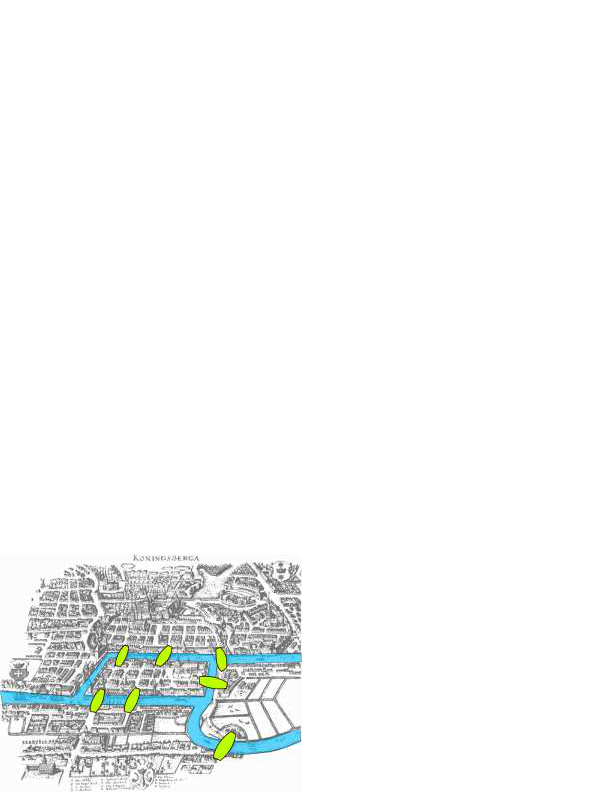
\includegraphics[width=5cm]{fig/sevenBridges.eps}
      \hspace{1cm}
      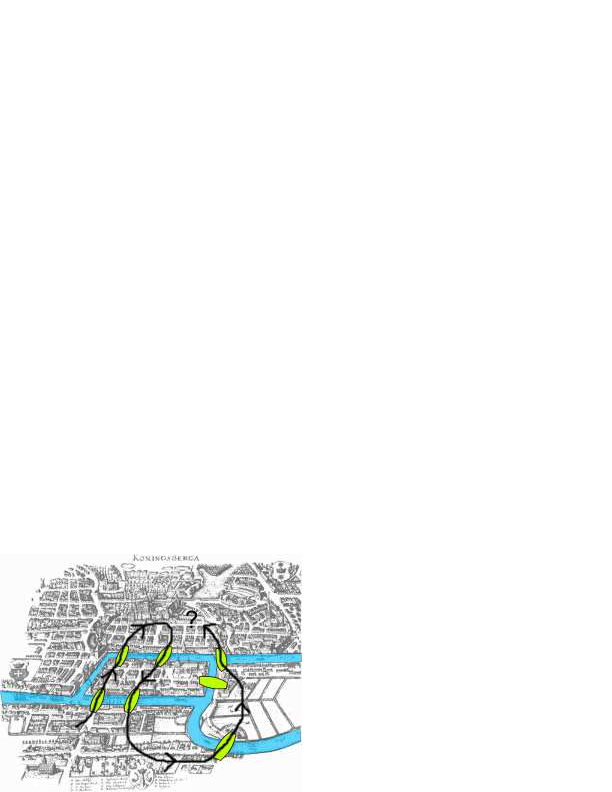
\includegraphics[width=5cm]{fig/sevenBridgesWrongWalk.eps} \\
   (A) \hspace{5.5cm} (B)\\
   \end{center}
   \vspace{-0.7cm}
   \caption{Seven bridges of K�nigsberg}
   \label{fig:sevenBridges}
\end{figure}

In the XVIII century, the city of K�nigsberg, Prussia (now
Kaliningrad, Russia) had seven bridges over the Pregel river
connecting two islands and other parts of the city as is shown in
Figure~\ref{fig:sevenBridges}A. A famous problem concerning
K�nigsberg was whether it was possible to take a walk through the
town in such a way as to cross over every bridge only one time.
Figure~\ref{fig:sevenBridges}B shows a wrong walk attempt: by the
time the sixth bridge is crossed the only uncrossed bridge is
unreachable.

No one was able to do this walk, and yet nobody knew how to prove
that it could not be done. In 1735, some college students sent this
problem to Leonhard Euler, one of the greatest mathematician of all
time. Euler was able to prove mathematically that this walk was
impossible. This result did not depend on the lengths of the
bridges, nor on their distance from one another, but only on
connectivity properties: which bridges are connected to which
islands or riverbanks. What Euler captured with the ``Problem of the
Seven Bridges of K�nigsberg'' is the motivating insight behind
topology:
\begin{center}\it
some geometric problems depend not on the exact shape of the objects
\linebreak involved, but rather on the ``way they are connected
together''.\end{center} Leonhard Euler's 1736 paper on Seven Bridges
of K�nigsberg is regarded as one of the first topological results
and also led to graph theory, a branch of mathematics with
``infinite'' applications
\cite{wiki:topology,wiki:sevenBridgesOfKonigsberg}.

Topology, in its present form, long after Euler, uses the term {\it
topological space} for what we called a ``shape'' on the beginning
of this section. Before defining what are {\it topological spaces}
we define {\it metric spaces}, as they are the source for the
concrete ``shapes'' or {\it topological spaces} that we are
interested.

\bigskip \centerline{\bf \textsc{Metric Spaces}} \bigskip

A {\it metric} or a {\it distance} in a set $X$ is a function $\rho:
X \times X \rightarrow \IR_+ = \{x \in \IR \, | \, x \geq 0 \}$ that
satisfies $$\begin{array}{l}
  \hbox{(1) \,} \rho(x,y) = 0, \hbox{ iff }x = y,\\[0.2cm]
  \hbox{(2) \,}\rho(x,y) = \rho(y,x), \hbox{ for every }x,y \in X,\\[0.2cm]
  \hbox{(3) \,}\rho(x,y) \leq \rho(x,z) + \rho(z,y), \hbox{ for every }x,y,z \in X. \hbox{ ({\it triangle inequality})}\\
\end{array}$$
The pair $(X,\rho)$, where $\rho$ is a metric in $X$, is called a
{\it metric space}. The function
$$\IR^n \times \IR^n \rightarrow \IR_{+} : (x,y) \mapsto
\sqrt{\sum_{i=1}^{n}{(x_i-y_i)^2}}$$ is a metric in $\IR^n$ and is
called {\it euclidean} metric.

Let $(X,\rho)$ be a metric space, let $a$ be a point in $X$, and let
$r$ be a positive real number. The sets
$$\begin{array}{l}
  B_r(a) = \{ x \in X \, | \, \rho(a,x) < r \},\\[0.2cm]
  D_r(a) = \{ x \in X \, | \, \rho(a,x) \leq r \},\\[0.2cm]
  S_r(a) = \{ x \in X \, | \, \rho(a,x) = r \}\\[0.2cm]
\end{array}$$
are called, respectively, {\it open ball}, {\it closed ball}, and
{\it sphere} of the space $(X,\rho)$ with center $a$ and radius $r$.
If $(X,\rho)$ is a metric space and $A \subset X$, then the
restriction of metric $\rho$ to $A \times A$ is a metric in $A$, and
$(A,\rho|_{A \times A})$ is a metric space. It is called a {\it
subspace} of $(X,\rho)$. The ball $D_1(0)$ and the sphere $S_1(0)$
in $\IR^n$ with the euclidean metric are denoted by symbols $D^n$
and $S^{n-1}$ and called {\it $n$-dimensional ball} and {\it
$(n-1)$-dimensional sphere}. They are considered as metric spaces
with the metric restricted to $\IR^n$. Note that: $D^1$ is the
segment $[-1,1]$; $D^2$ is a disk; $S^0$ is the pair of points
\{-1,1\}; $\IS^1$ is a circle; $\IS^2$ is a sphere; $D^3$ is a ball. The
words disk, circle, sphere and ball were used, in last sentence,
appealing to their common sense meaning. Now, for this work,
they have a formal meaning: a {\it disk} is $D^2$, a {\it circle} is
$\IS^1$, a {\it sphere} is $\IS^2$ and a {\it ball} is $B^3$.

\newpage

\bigskip \centerline{\bf \textsc{Topological Spaces}} \bigskip

A {\it topological space} is a set $X$ with a collection $\Omega$ of
subsets of $X$ satisfying the following three axioms:

\smallskip

\begin{tabular}{l}
(1) \,\, the empty set $\varnothing$ and $X$ are in $\Omega$, \\[0.2cm]
(2) \,\, the union of any collection of sets in $\Omega$ is in $\Omega$, \\[0.2cm]
(3) \,\, the intersection of any pair of sets in $\Omega$ is in $\Omega$. \\[0.2cm]
\end{tabular}

The collection $\Omega$ is called a {\it topological structure} or a
{\it topology} in $X$. The sets in $\Omega$ are called {\it open}.
The elements of $X$ are called {\it points}. A set $F \in X$ is said
{\it closed} in the space $(X,\Omega)$ if its complement $X
\backslash F$ is open ({\it i.e. $X \backslash F \in \Omega$}). Note
that $\varnothing$ and $X$ are both open and closed. A {\it
neighborhood} of a point is any open set containing that point. A
collection $\Sigma$ of open sets is called a {\it base} for a
topology ({\it i.e.} topological structure), if each nonempty open
set is a union of sets belonging to $\Sigma$.

The following result connects metric spaces and topological spaces:
\begin{center}
\it the collection of all open balls in a metric space $(X,\rho)$
\linebreak is a base for some topology in $X$.
\end{center}
For example, consider $\IR^2$ with the euclidean metric. Then, a
topology for $\IR^2$ is the set of all unions of open balls (open
disks in the plane). This topology is the default topology when
nothing else is mentioned.

Let $(X,\Omega)$ be a topological space, and $A \subset X$. Denote
by $\Omega_A$ the collection of sets $A \cap V$, where $V \in
\Omega$. Then,
\begin{center} \it
$\Omega_A$ is a topological structure in $A$.
\end{center}
The pair $(A,\Omega_A)$ is called a {\it subspace} of the space
$(X,\Omega)$. The collection $\Omega_A$ is called the {\it subspace
topology} or the topology {\it induced} on $A$ by $\Omega$, and its
elements are the open sets in $A$.

At this point, we can think, for instance, of $\IS^2$ as a topological
space. We know that the collection of open balls of $\IR^3$ (as a
metric space with the euclidean metric) is a base for a topology in
$\IR^3$. Consider this topology to view $\IR^3$ as a topological
space. Restrict this topology of $\IR^3$ to $\IS^2$ to obtain a
topology for $\IS^2$: $\IS^2$ is now a topological space. In this work
this logical sequence to obtain a topology for a subset of $\IR^n$
is always the one considered. So, from now on, every subset of
$\IR^n$ may also be viewed as a topological space. For example the
surface of doughnut and of the coffee cup considered in the
beginning of this section may now be viewed as subsets of $\IR^3$
and, consequently, as topological spaces.

\bigskip \centerline{\bf \textsc{Maps}} \bigskip

In the context of topology, the terms {\it map} and {\it mapping}
are synonyms of function. A mapping $f: X \rightarrow Y$ is called a
{\it surjective map}, or just a {\it surjection} if every element of
$Y$ is an image of at least one element of $X$. It is called an {\it
injective map}, {\it injection} or {\it one-to-one map} if every
element of $Y$ is an image of, at most, one element of $X$. A
mapping is called a {\it bijective map}, {\it bijection}, or {\it
invertible} if it is surjective and injective.

The {\it image} of a set $A \subset X$ under a map $f: X \rightarrow
Y$ is the set of images of all points of $A$. It is denoted by
$f(A)$. Thus,
$$f(A) = \{ f(x) : x \in A \}.$$
The image of the entire set $X$ ({\it i.e.} $f(X)$) is called the
{\it image} of $f$. The {\it preimage} of a subset of $B \subset Y$
under map $f: X \rightarrow Y$ is the set of elements of $X$ whose
images belong to $B$. It is denoted by $f^{-1}(B)$. Thus,
$$f^{-1}(B) = \{ x : f(x) \in B \}.$$

\bigskip \centerline{\bf \textsc{Continuous Maps}} \bigskip

Let $X$, $Y$ be topological spaces. A map $f:X \rightarrow Y$ is
said to be {\it continuous} if the preimage of any open subset of
$Y$ is an open subset of $X$. A map $f:X \rightarrow Y$ is said to
be {\it continuous at point }$a \in X$ if for every neighborhood $U$
of $f(a)$ there exists a neighborhood $V$ of $a$ such that $f(V)
\subset U$. One result about continuous maps is that: a map $f:X
\rightarrow Y$ is continuous iff it is continuous at each point of
$X$. Another result is that this notion of continuity coincides with
the one that is usually studied in calculus:
\begin{center} {\it
Let $X, Y$ be metric spaces, and $a \in X$. A map $f:X \rightarrow
Y$ is \linebreak continuous at the point $a$, iff for every
$\epsilon
> 0$ there exists a $\delta > 0$ \linebreak such that for every point $x \in X$
inequality  $\rho(x,a) < \delta$ implies \linebreak
$\rho(f(x),f(a))<\epsilon$.}
\end{center}

\bigskip \centerline{\bf \textsc{Homeomorphism}} \bigskip

Now we are able to formally define the ``topologically equivalence''
concept. An invertible mapping is called a {\it homeomorphism} if it
is continuous and its inverse is also continuous. A topological
space $X$ is said to be {\it homeomorphic} to space $Y$ if there is
a homeomorphism $X \rightarrow Y$. Being homeomorphic is {\it an
equivalence relation}. Let $X$, $Y$ and $Z$ be topological spaces
then: (1) $X$ is homeomorphic to $X$; (2) if $X$ is homeomorphic to
$Y$ then $Y$ is homeomorphic to $X$; and (3) if $X$ is homeomorphic to
$Y$ and $Y$ is homeomorphic to $Z$ then $X$ is homeomorphic to $Z$.

Some examples of homeomorphic topological spaces: $[0,1]$ and
$[a,b]$ for any $a < b$; $(-1,1)$ and $\IR$; an open disk and the
plane $\IR^2$; $\IS^n \backslash \{\hbox{point in }\IS^n\}$ and $\IR^n$.
Some examples of non-homeomorphic topological spaces: balls $D^p,
D^q$ with $p \neq q$; spheres $S^p, S^q$ with $p \neq q$; punctured
plane $\IR^2 \backslash \{\hbox{point}\}$ and a plane with a hole
$\IR^2 \backslash \{(x,y):x^2+y^2<1\}$.

From the topological point of view homeomorphic spaces are
completely identical: a homeomorphism $X \rightarrow Y$ establishes
one-to-one correspondence between all phenomena in $X$ and $Y$ which
can be expressed in terms of topological structures. Thus, two
spaces are {\it topologically equivalent} or {\it the same for the
purposes of topology} if there is a homeomorphism between them.
There is a homeomorphism between the surface of a doughnut and the
surface of a coffee cup, so they are topologically equivalent.

As we pointed out on the first paragraph of this section, not yet in
the correct language, the topological equivalence problem or {\it
homeomorphism problem} is one of the classic and important problems
of topology:
\begin{center}
\it Given two topological spaces, are they homeomorphic?
\end{center}
To prove that topological spaces are homeomorphic, it is enough to
present a homeomorphism between them. Essentially this is what is
done in this case. However, to prove that topological spaces are not
homeomorphic, it does not suffice to consider any special mapping,
and is usually impossible to review all mappings. Therefore for proving
non-existence of a homeomorphism one uses indirect arguments. In
particular, one finds a property or a characteristic shared by
homeomorphic spaces such that one of the spaces has it, while the
other does not. Properties and characteristics shared by homeomorphic
spaces are called {\it topological properties} or {\it invariants}. For instance, the
cardinality of the set of points and of the set of open sets is a
topological invariant.

\bigskip \centerline{\bf \textsc{Embedding}} \bigskip

A continuous mapping $f: X \rightarrow Y$ is called a {\it
(topological) embedding} if the mapping \hbox{$f':X \rightarrow
f(X)$} is a homeomorphism, where $f'(x) = f(x)$ for all $x \in X$.
Embeddings $f_1, f_2: X \rightarrow Y$ are said to be {\it
equivalent} if there exist homeomorphisms $h_X:X \rightarrow X$ and
$h_Y:Y \rightarrow Y$ such that $f_2 \circ h_X = h_Y \circ f_1$.

Note that homeomorphisms are special kind of embeddings, where the
mapping is surjective.

\bigskip \centerline{\bf \textsc{Cover}} \bigskip

A collection $\Gamma$ of subsets of a set $X$ is called a {\it
cover} or a {\it covering} if the union of the elements of
$\Gamma$ contains $X$, {\it i.e.}, $X \subset \cup_{A \in \Gamma}A$.
A cover $\Gamma$ of a topological space $X$ is said to be an {\it
open cover} if every element of $\Gamma$ is an open set. A cover
$\Gamma$ of a topological space $X$ is said to be a {\it closed
cover} if every element of $\Gamma$ is a closed set. If $\Sigma$
covers $X$ and $\Gamma$ covers $X$ and $\Sigma \subset \Gamma$, then
$\Sigma$ is a {\it subcover} or {\it subcovering} of $\Gamma$.

\begin{comment}
if $X$ is a union of sets belonging to $\Gamma$, {\it i.e}, of
belonging to .., i.e., X = SA... A. In this case elements of .. are
said to cover X. There is also a more general meaning of these
words. A collection .. of subsets of a set Y is called a cover or a
covering of a set X . Y if X is contained in the union of the sets
belonging to .., i.e., X . SA... A. In this case, sets belonging to
.. are also said to cover X. �9.11 Fundamental Covers Consider a
cover .. of a topological space X. Each element of .. inherits from
X a topological structure. When are these structures sufficient for
recovering the topology of X? In particular, under what conditions
on .. does continuity of a map f : X . Y follow from continuity of
its restrictions to elements of ... To answer these questions, solve
the problems 9.28�9.29 and 9.Q�9.V. 9.28. Is this true for the
following coverings: (a) X = [0, 2], .. = {[0, 1], (1, 2]}; (b) X =
[0, 2], .. = {[0, 1], [1, 2]}; (c) X = R, .. = {Q,R r Q}; (d) X = R,
.. is a set of all one-point subsets of R? 9.29. A cover of a
topological space consisting of one-point subsets has the property
described above, iff the space is discrete. A cover .. of a space X
is said to be fundamental if a set U . X is open, iff for every A .
.. the set U n A is open in A. 9.Q. A covering .. of a space X is
fundamental, iff a set U . X is open provided U n A is open in A for
every A . ... 9.R. A covering .. of a space X is fundamental, iff a
set F . X is closed provided F n A is closed A for every A . ... A
{\it cover} of a set $X$ is a collection $\Gamma$ of subsets of $X$
such that their union is equal to $X$. If $X$ is a topological
space, a
\end{comment}

\bigskip \centerline{\bf \textsc{Connectedness}} \bigskip

A topological space $X$ is said to be {\it connected} if it has only
two subsets which are both open and closed: $\varnothing$ and the
entire $X$. Although this definition is clear, at first, it is not
intuitive. Let's get a more intuitive definition. A {\it partition}
of a set is a cover of this set with pairwise disjoint sets. To {\it
partition} a set means to construct such a cover. Now the equivalent
notion of connectedness of a topological space:
\begin{center}
\it A topological space is connected iff it cannot be \linebreak
partitioned into two nonempty open sets iff it cannot be \linebreak
partitioned into two nonempty closed sets.
\end{center}
For instance, consider the topological space obtained as a subspace
of the plane that consists of two disjoint open disks (open balls)
({\it e.g}: one open ball $B_1(-1,-1)$ and $B_1(1,1)$). This
topological space is not connected, because the two open disks, that
are open sets, form a partition of the entire space.

A {\it connected component} of a space $X$ is a maximal connected
subset of $X$ ({\it i.e.} a connected subset, that is not contained
strictly in other larger subset of $X$). Some properties of
connected components: every point belongs to some connected
component; connected components are closed; two connected
components are disjoint or coincident. The image of a connected
space under a continuous mapping is connected, so connectedness is a
topological property. The number of connected components is a
topological invariant.

\bigskip \centerline{\bf \textsc{Compactness}} \bigskip

A topological space $X$ is said to be {\it compact} if any of its
open covers has a finite subcover, {\it i.e.} if $\Gamma$ is a cover
for $X$ then exists a finite $\Sigma \subset \Gamma$ that also
covers $X$. The image of a compact space by a continuous mapping is
also compact, so compactness is a topological property.

Compactness is a sort of topological counter-part for the property
of being finite in the context of set theory. Example of s non-compact
space: $\IR^n$. Example of a compact space: $\IS^n$. Indeed a subset of $\IR^n$ is compact
if and only if it is closed and bounded (\ie contained in an open ball).



\bigskip \centerline{\bf \textsc{Homotopy}} \bigskip

Let $f, g$ be continuous maps of a topological space $X$ to a
topological space $Y$, and $H: X \times [0,1] \rightarrow Y$ a
continuous map such that $H(x,0) = f(x)$ and $H(x,1) = g(x)$ for any
$x \in X$. Then $f$ and $g$ are said to be {\it homotopic} and $H$
is called a {\it homotopy} between $f$ and $g$. Homotopy of maps is
an equivalence relation: (1) if $f: X \rightarrow Y$ is a continuous
map then $H:X \times [0,1] \rightarrow Y$ defined by $H(x,t) = f(x)$
is a homotopy between $f$ and $f$; (2) if $H$ is a homotopy between
$f$ and $g$ then $H'$ defined by $H'(x,t) = H(x,1-t)$ is a homotopy
between $g$ and $f$; (3) if $H$ is a homotopy between $f$ and $f'$
and $H'$ is a homotopy between $f'$ and $f''$ then $H''$ defined by
$$ H''(x,t) =
 \left\{
 \begin{array}{ll}
 H(x,2t) & \hbox{for } t \leq 1/2,\\
 H'(x,2t-1) & \hbox{for } t \geq 1/2,\\
 \end{array}\right.$$ is a homotopy between $f$ and $f''$.

\bigskip \centerline{\bf \textsc{Isotopy}} \bigskip

Let $X$, $Y$ be topological spaces, $h, h': X \rightarrow Y$
homeomorphisms. A homotopy $h_t:X \rightarrow Y$, $t \in [0,1]$
connecting $h$ and $h'$ ({\it i.e.}, with $h_0 = h$, $h_1 = h'$) is
called a {\it isotopy} between $h$ and $h'$ if $h_t$ is a
homeomorphism for each $t \in [0,1]$. Homeomorphisms $h, h'$ are
said to be {\it isotopic} if there exists an isotopy between $h$ and
$h'$. Being isotopic is an equivalence relation on the set of
homeomorphisms $X \rightarrow Y$.

The concept of isotopy may also be applied to embeddings. Let $X$,
$Y$ be topological spaces, $h, h': X \rightarrow Y$ topological
embeddings. A homotopy $h_t:X \rightarrow Y$, $t \in [0,1]$
connecting $h$ and $h'$ ({\it i.e.}, with $h_0 = h$, $h_1 = h'$) is
called an {\it (embedding) isotopy} between $h$ and $h'$ if $h_t$ is
an embedding for each $t \in [0,1]$. Embeddings $h, h'$ are said to
be {\it isotopic} if there exists an isotopy between $h$ and $h'$.
Being isotopic is an equivalence relation on the set of embeddings
$X \rightarrow Y$.

A family $A_t$, $t \in I = [0,1]$ of subsets of a topological space
is called an {\it isotopy of the set $A = A_0$} if the graph $\Gamma
= \{(x,t) \in X \times I \, | \, x \in A_t\}$ of the family is {\it
fibrewise homeomorphic} to the cylinder $A \times I$, {\it i.e.}
there exists homeomorphisms $A \times I \rightarrow \Gamma$ mapping
$A \times \{t\}$ to $\Gamma \cap X \times \{t\}$ for any $t \in I$.
Such a homeomorphism gives rise to an isotopy of embeddings $ \Phi_t
: A \rightarrow X$, $t \in I$ where $\Phi_0$ is the identity mapping
and $\Phi_t(A) = A_t$. An isotopy of a subset is also called a {\it
subset isotopy}. Subsets $A$ and $A'$ of the same topological space
are said to be {\it isotopic in $X$}, if there exists a subset
isotopy $A_t$ of $A$ with $A' = A_1$. The isotopic relation over the
set of subsets of a topological space $X$ is an equivalence
relation.

An isotopy of a subset $A \in X$ is said to be {\it ambient}, if it
may be accompanied with an embedding isotopy $\Phi_t : A \rightarrow
X$ extendible to an isotopy $\tilde{\Phi_t}: X \rightarrow X$ of the
identity homeomorphism of space $X$. The isotopy $\tilde{\Phi_t}$ is
said to be {\it ambient} for $\Phi_t$. Two isotopic subsets of a
topological space may not be ambient isotopic. Any pair of circles
$\IS^1$ embedded in $\IS^3$ is isotopic, but a circle
(Figures~\ref{fig:links3d}A) and a trefoil
(Figures~\ref{fig:links3d}B) are not ambient isotopic.

\bigskip \centerline{\bf \textsc{Manifolds}} \bigskip

Let $n$ be a non-negative integer. A topological space $X$ is called
{\it locally euclidean space of dimension $n$} if each point of $X$
has a neighborhood homeomorphic either to $\IR^n$ or $\IR^n_{+}$
({\it i.e.} $\IR^n_+ = \{ x \in \IR^n : x_1 \geq 0 \}$, defined for
$n \geq 1$). Examples of locally euclidean spaces: $\IR^n$; $\IS^n$,
$D^n$.

A topological space is called {\it Hausdorff space} or just {\it
Hausdorff} if any two distinct points possess disjoint
neighborhoods. Result: any metric space is Hausdorff ({\it i.e.} the
topological space with topology induced from the metric space is
Hausdorff).

A space is said to satisfy the {\it second axiom of
countability} or to be {\it second countable} if it has a countable
base. Result: any metric space is Hausdorff ({\it i.e.} the
topological space with topology induced from the metric space has
a countable base).

A {\it manifold of dimension $n$} or $n$-manifold is a topological
space that satisfies:
\smallskip

\begin{tabular}{l}
(1) \,\, it is a locally euclidean space of dimension $n$, \\[0.2cm]
(2) \,\, it is Hausdorff, \\[0.2cm]
(3) \,\, it is second countable. \\[0.2cm]
\end{tabular}

\smallskip

Examples of {\it $n$-manifolds}: $\IR^n$; $\IS^n$, $D^n$.

The definitions until now were very formal, but this one will not be
formal. A manifold of dimension $n$ is called {\it non-orientable}
if it is possible to take the homeomorphic image of an
\hbox{$n$-dimensional} ball in the manifold and move it through the
manifold and back to itself, so that at the end of the path, the
ball has been reflected. The M�bius band and Klein bottle are the
most famous examples of non-orientable manifolds. A manifold which
is not non-orientable is {\it orientable}. An orientable space has
two orientations and the choice of one of them makes the space an
{\it oriented} space.

\bigskip \centerline{\bf \textsc{Spaces for us$\ldots...$}} \bigskip

In this work we are interested in studying a specific kind of
``shape'' or, as we learned, topological space. This is it:
\begin{center}
\it \large connected, closed, oriented 3-manifolds.
\end{center}
The adjective {\em closed} applied to a 3-manifold means that it is boundary free and compact.
We use, from now on, the word {\it space} to denote these
topological spaces. This is not a perfect choice, as ``space'', even
in mathematics, has a lot of meanings. It could be a metric space. A
vector space. A topological space not matching these constraints of
being compact, connected, oriented. A common use for space, for
instance, is any 3-dimensional topological space or any 3-manifold.
These include our spaces but others too. In spite of all these,
here, space will be exactly this: a connected, compact, oriented
3-manifold. So let's put it big:
\begin{center}
\it \large A {\huge space} in this work is the same as \linebreak a
connected, closed, oriented 3-manifold.
\end{center}

\newpage

\section{Knots, links and diagrams}
\label{sec:knotsAndLinks}

In general terms, {\it knot theory} studies the {\it placement
problem}. As stated in \cite{Kauffman1987}, this problem is
\begin{center}
\it Given topological spaces $X$ and $Y$, classify how $X$ may be
\linebreak placed within $Y$. Here the ``how'' is usually an
 embedding, and classify often \linebreak means up to some form of
movement of $X$ in $Y$ (isotopy, for example).
\end{center} When $X$ is the circle $\IS^1$ and $Y$ is
the 3-dimensional space $\IR^3$ or $\IS^3$, we have {\it classical
knot theory}. In this section we see, for this classical knot
theory, a characterization of what are the equivalent embeddings.
Things shown here form the basis for the approach to the problem of
characterizing homeomorphic spaces (connected, compact, oriented
3-manifolds) that we show later.

An embedding of a circle $\IS^1$ in the 3-dimensional space $\IR^3$ or
in the 3-sphere $\IS^3$ is called a {\it knot}. An embedding of a
collection of circles in the 3-dimensional space $\IR^3$ or in the
3-sphere $\IS^3$ is called a {\it link}. Each circle (or the image of
one) in a link is called a {\it component} of the link. So, a knot
is a link with only one component. Figure \ref{fig:links3d} shows
some links\footnote{These figures were created using the beautiful
tool called \textsc{KnotPlot} that was part of the phd thesis of
Robert Scharein \cite{Scharein1998}.}. The link of Figure
\ref{fig:links3d}A is also a knot (one component) and is
suggestively called {\it unknot}. Figure \ref{fig:links3d}B is the
knot called {\it trefoil}. Figure \ref{fig:links3d}C is the knot
called {\it figure eight knot}. Figure \ref{fig:links3d}D is a
link with two components. Figure \ref{fig:links3d}E is a link with
three components and it is called the {\it borromean rings}. This link has
an interesting property: we cannot separate the three rings without
breaking one of them, {\it i.e.} the three rings are {\it linked},
even though, any two rings are separable without breaking ({\it
i.e.} any pair of rings is unlinked).

\begin{figure}[htp]
   \begin{center}
\begin{tabular}{ccccc}
      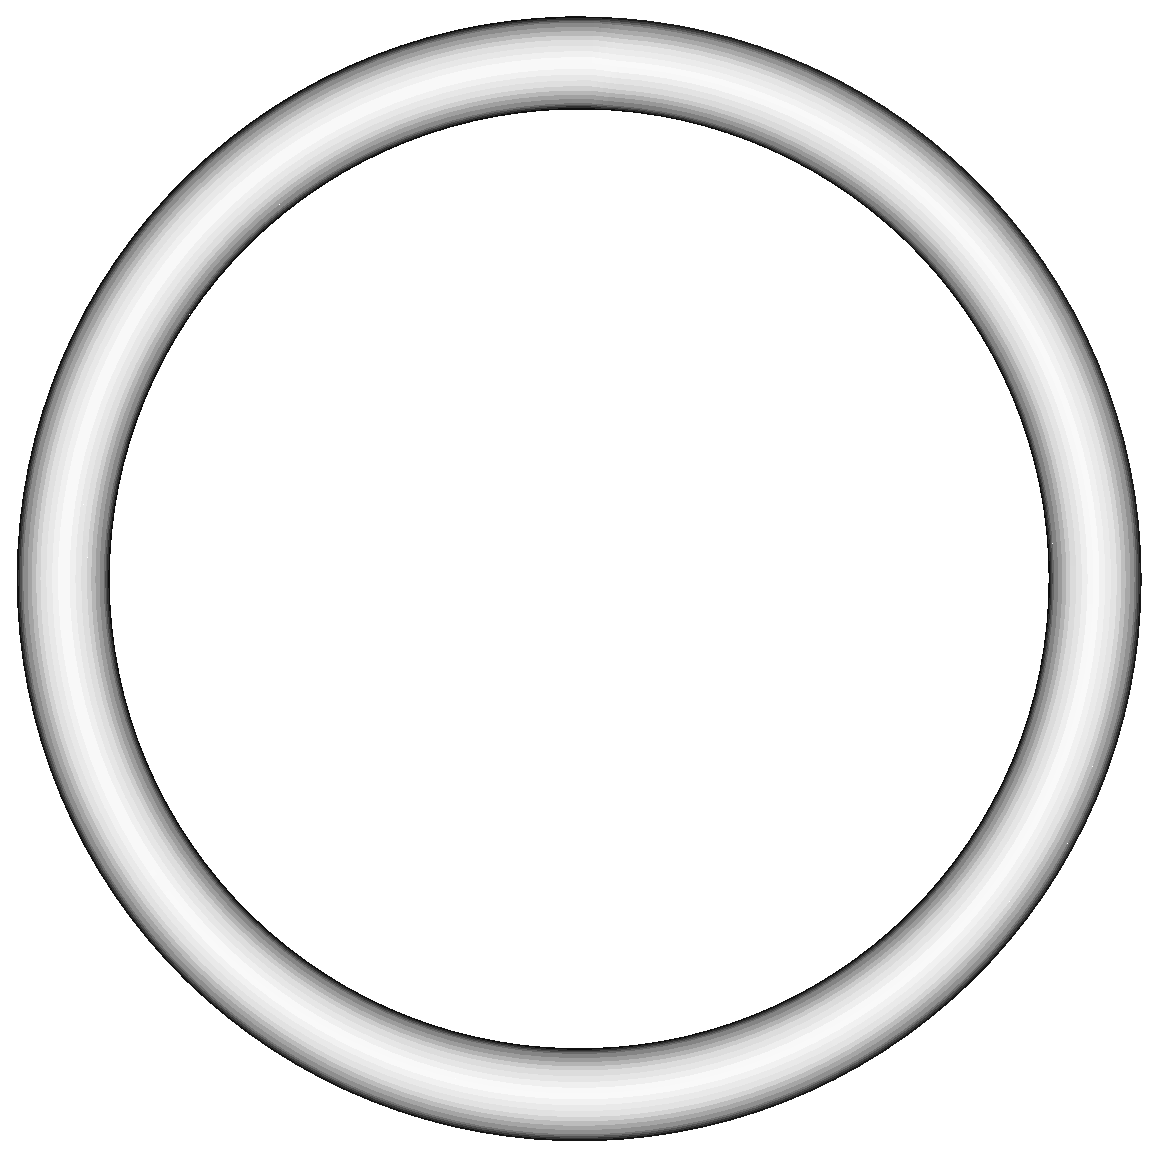
\includegraphics[width=2.5cm]{fig/link0.1.eps} &
      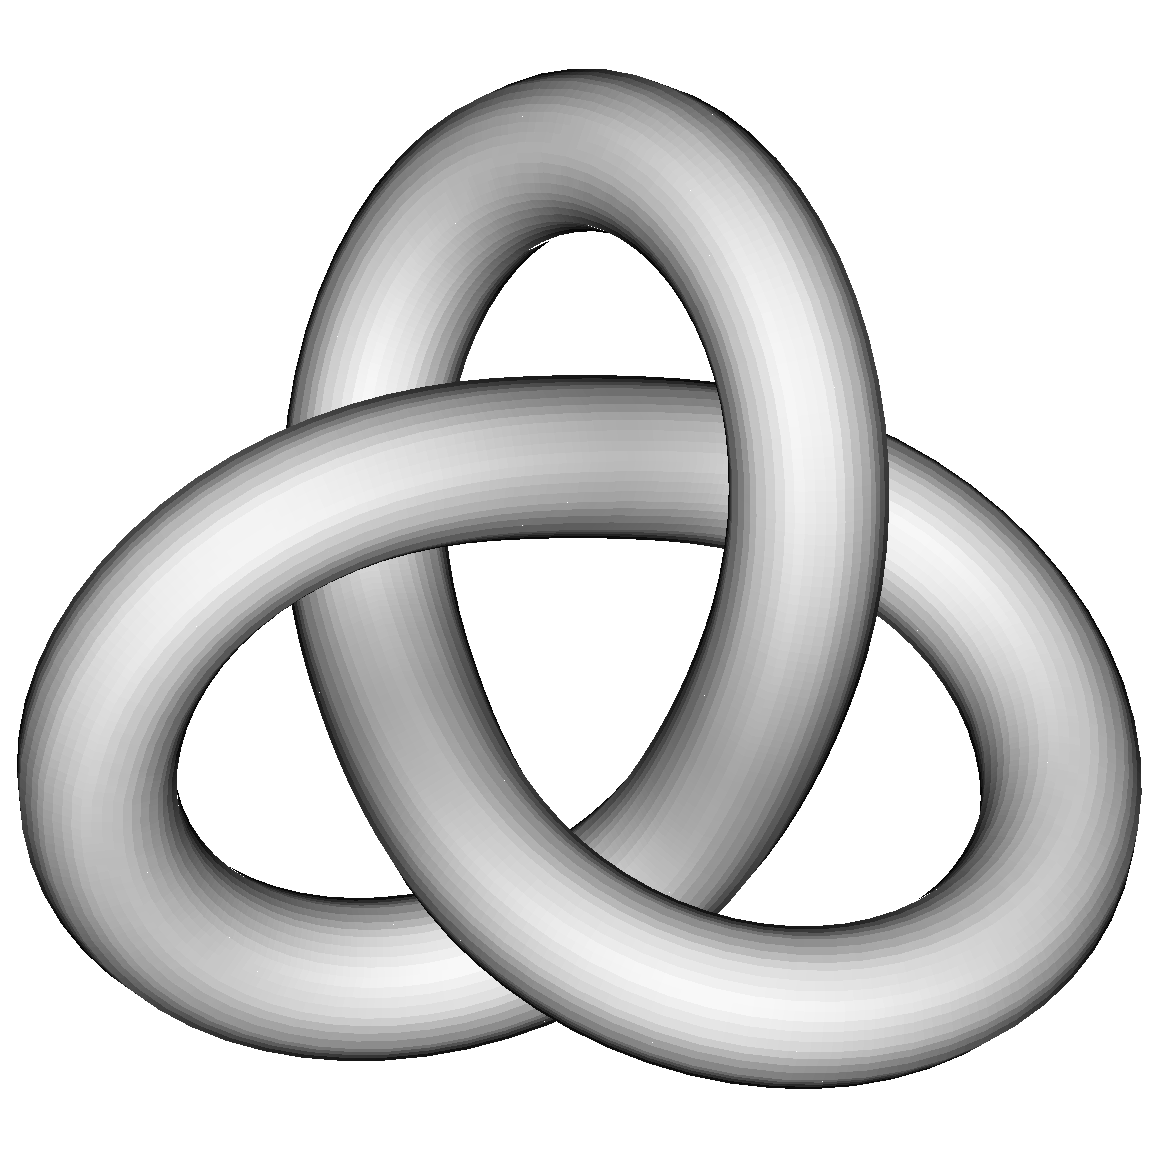
\includegraphics[width=2.5cm]{fig/link3.1.eps} &
      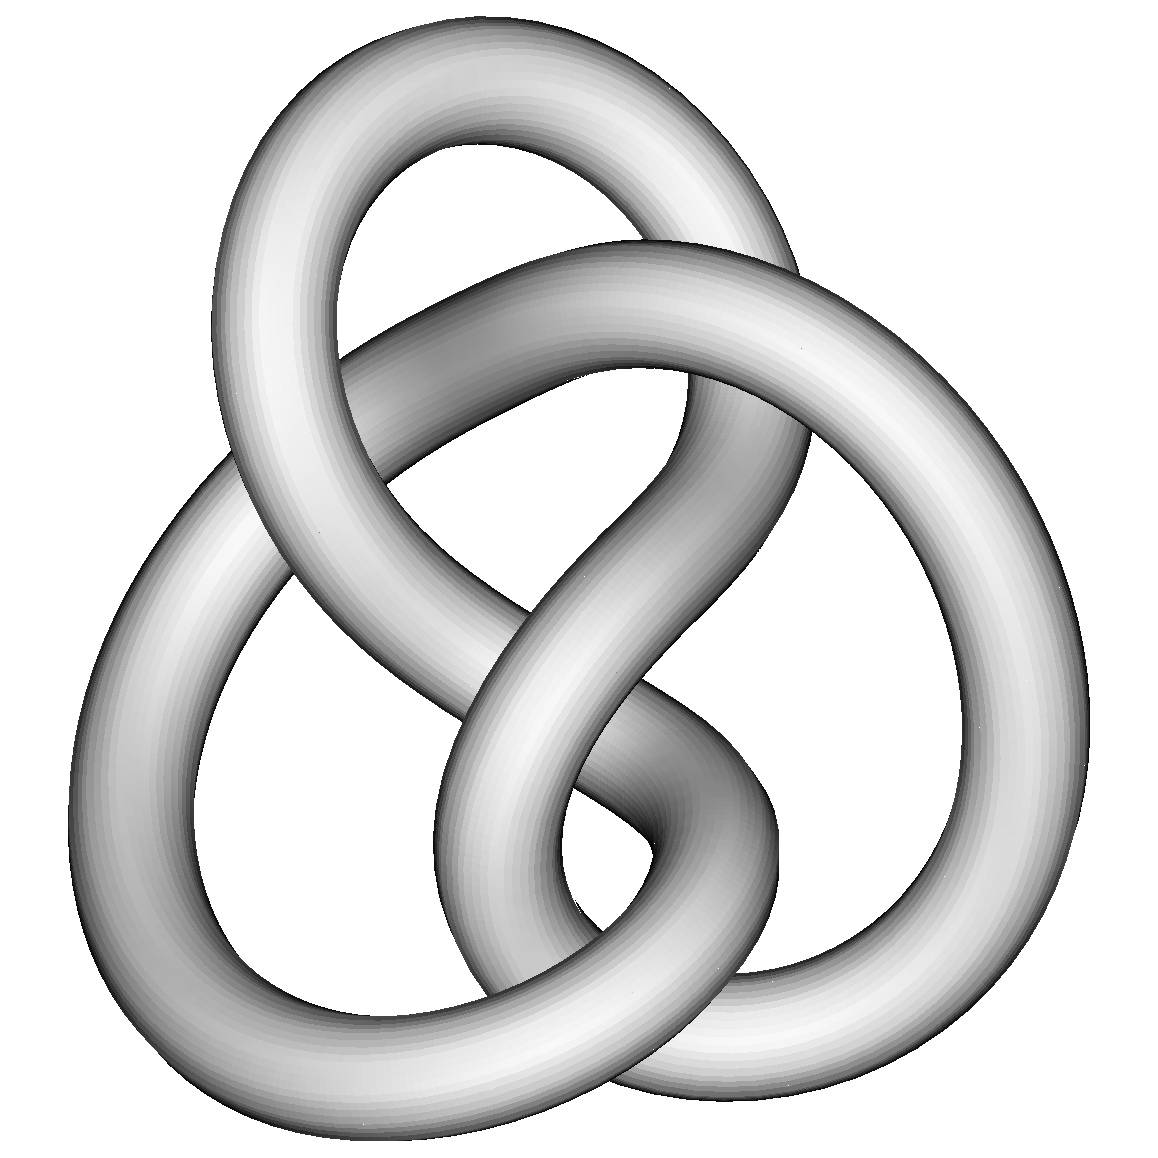
\includegraphics[width=2.5cm]{fig/link4.1.eps} &
      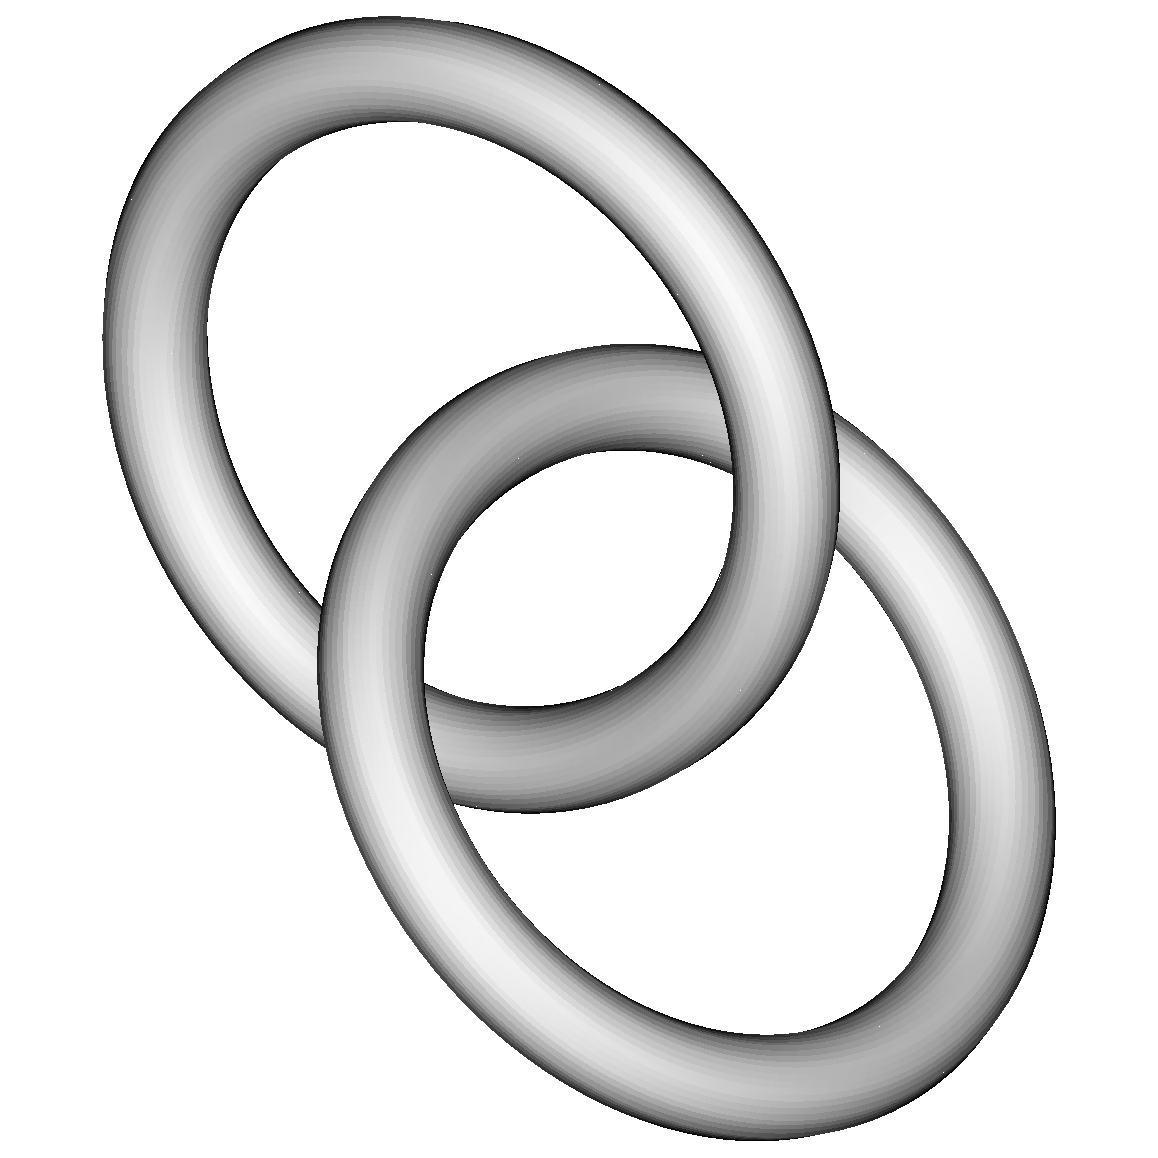
\includegraphics[width=2.5cm]{fig/2rings.eps} &
      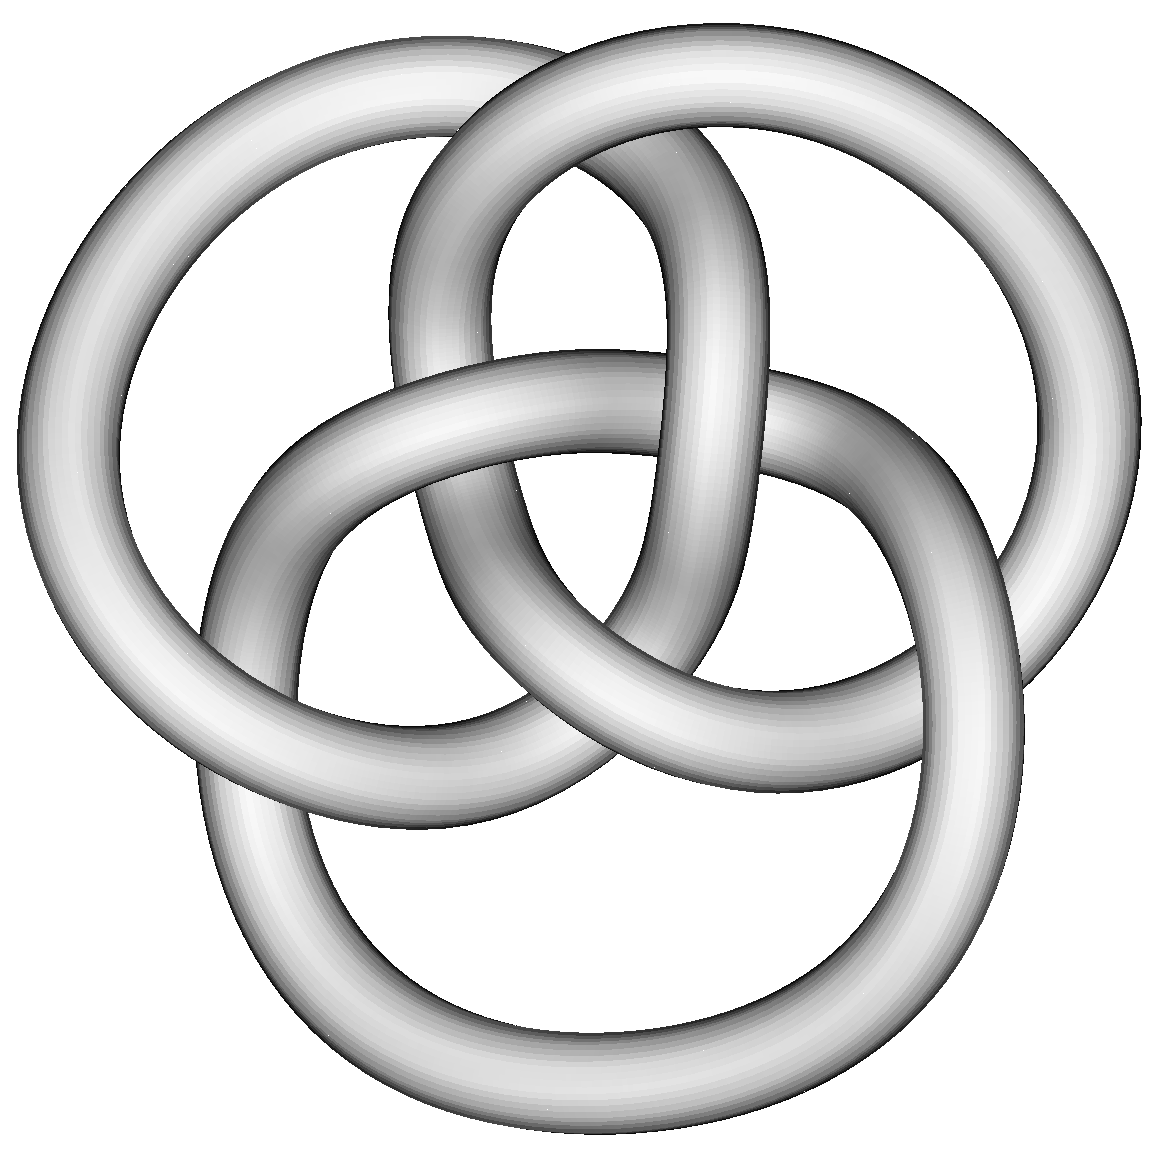
\includegraphics[width=2.5cm]{fig/borromean.eps} \\
      (A) & (B) & (C) & (D) & (E) \\
\end{tabular}
   \end{center}
   \vspace{-0.7cm}
   \caption{ Knots and links}
   \label{fig:links3d}
\end{figure}

Actually, Figure \ref{fig:links3d} presents the projection on the
``plane of this paper'' of thin cylinders centered and following the
1-dimensional strings that are the 3-dimensional image of the
circles through the embeddings or links. It happens that we could
replace Figure \ref{fig:links3d} by Figure \ref{fig:links3ddiagrams}
without loosing any important information. Each of this drawings is
called a {\it knot diagram} (if only one component) or {\it link
diagram} (any number of components). On each crossing that appears
in the plane projection of the cylinders, there is one cylinder
segment on top of another cylinder segment. This is represented by a
continuous curve (top segment) and a broken curve (bottom segment).

\begin{figure}[htp]
   \begin{center}
\begin{tabular}{ccccc}
      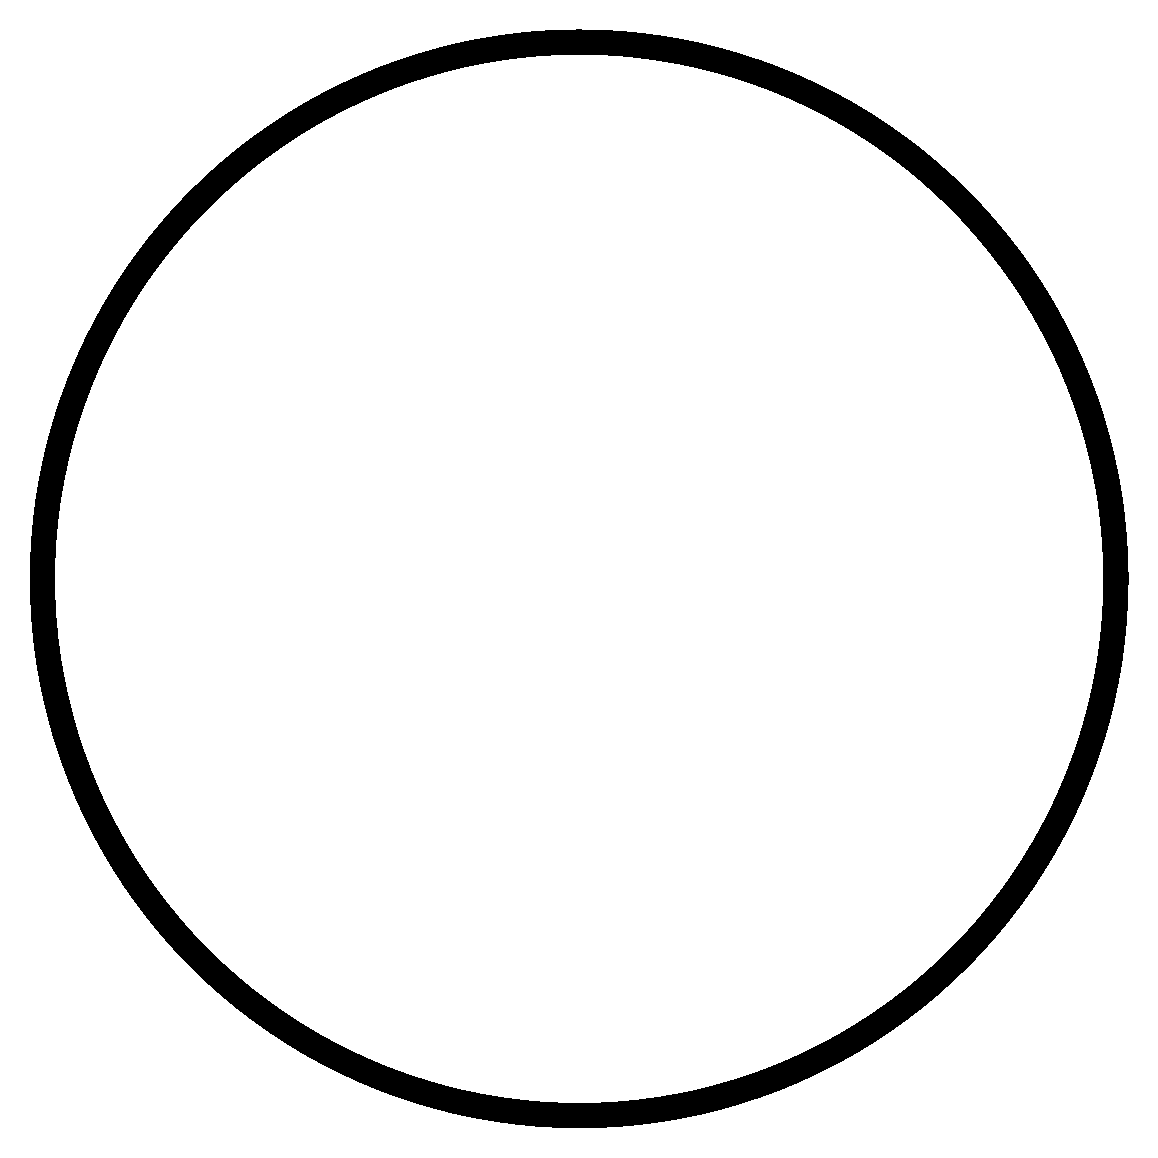
\includegraphics[width=2.5cm]{fig/link0.1d.eps} &
      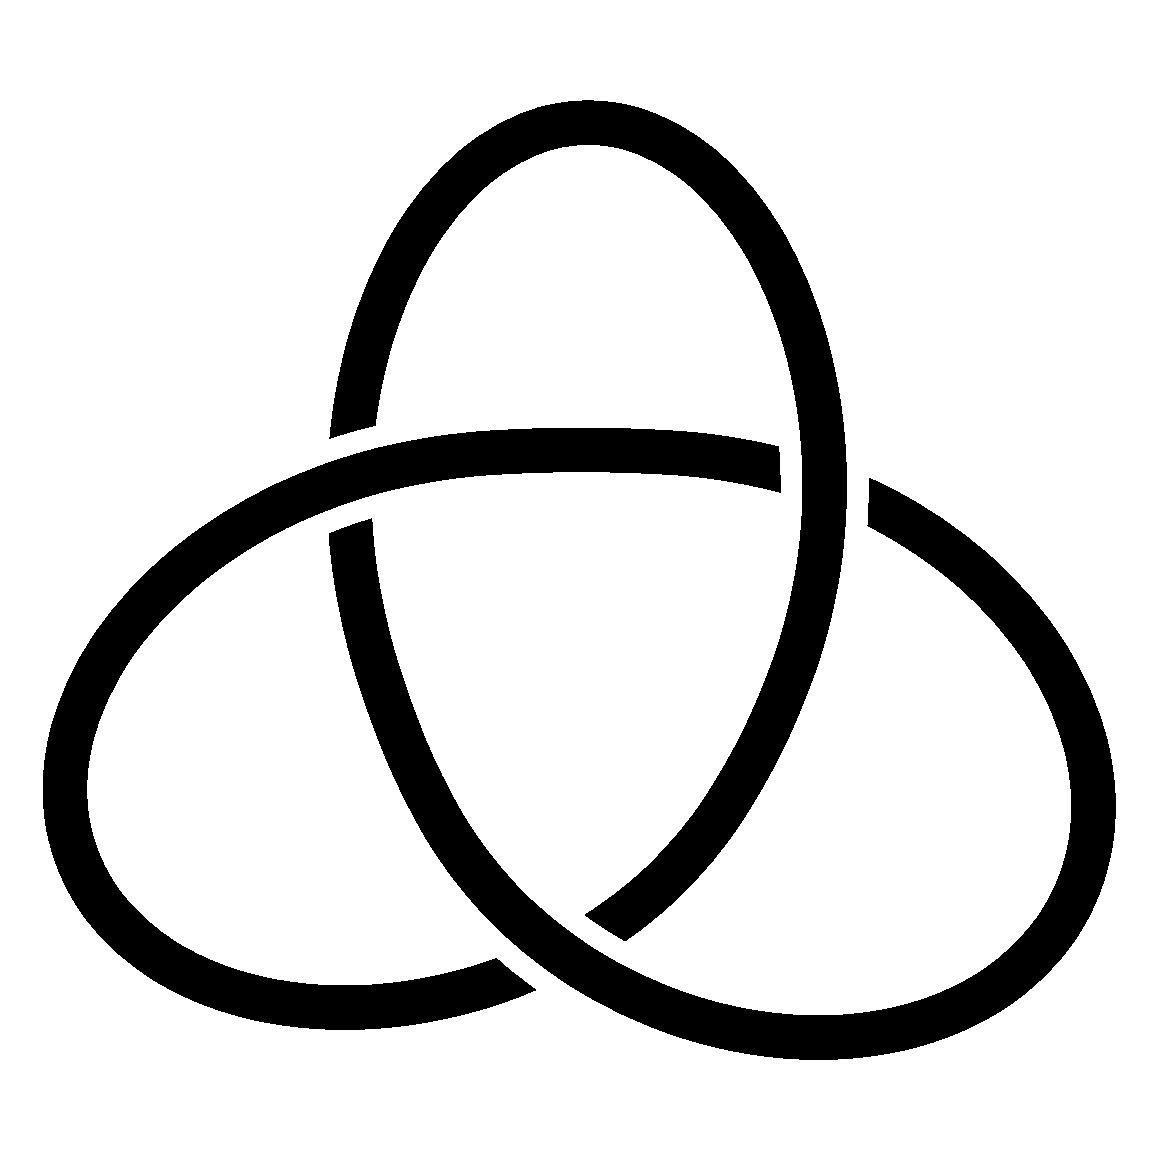
\includegraphics[width=2.5cm]{fig/link3.1d.eps} &
      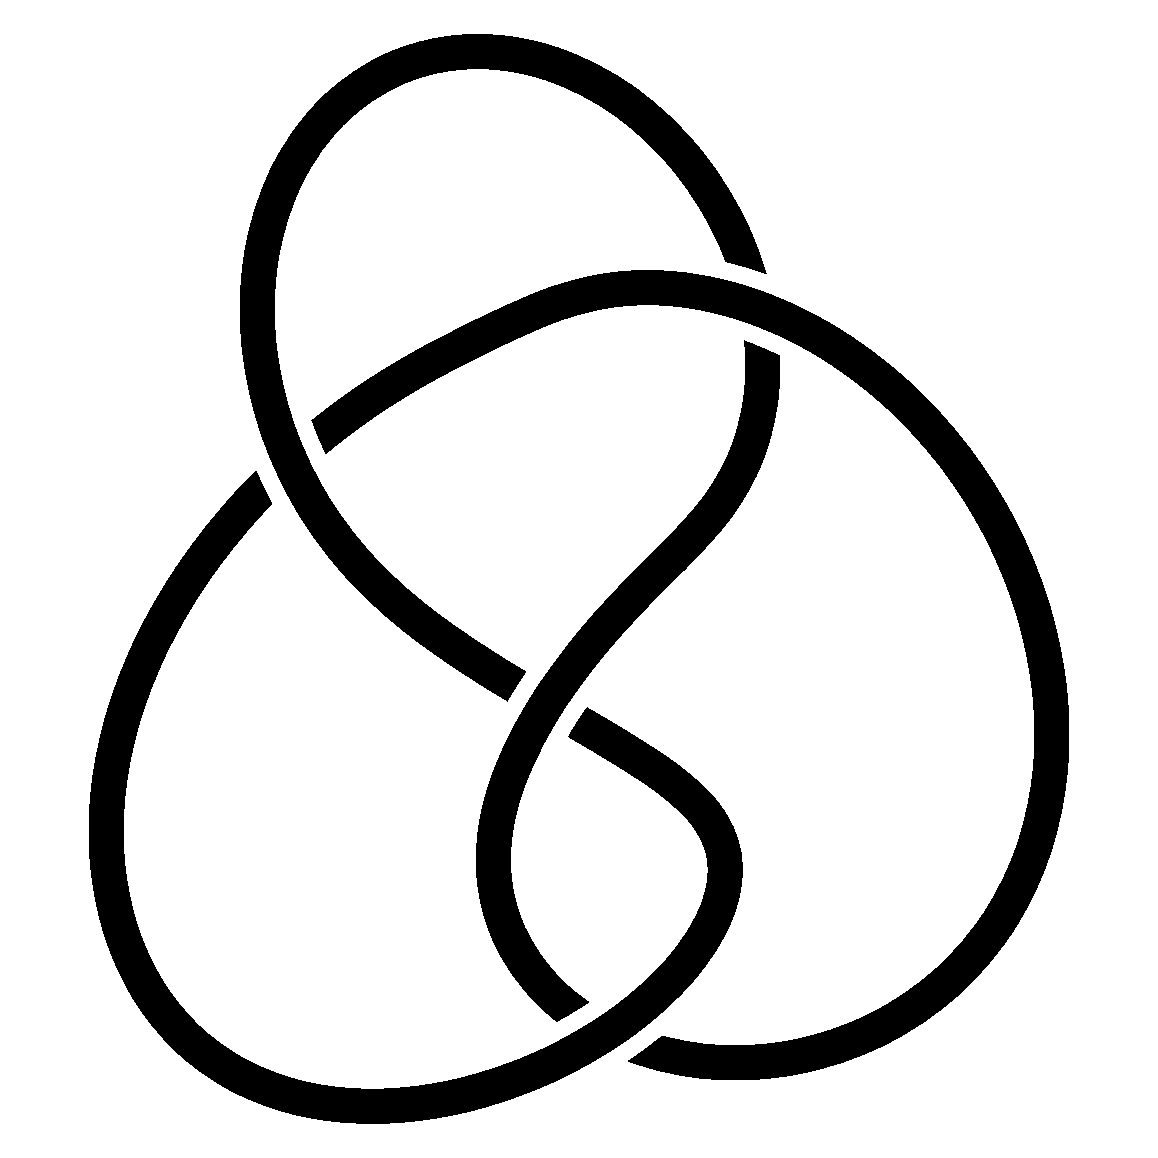
\includegraphics[width=2.5cm]{fig/link4.1d.eps} &
      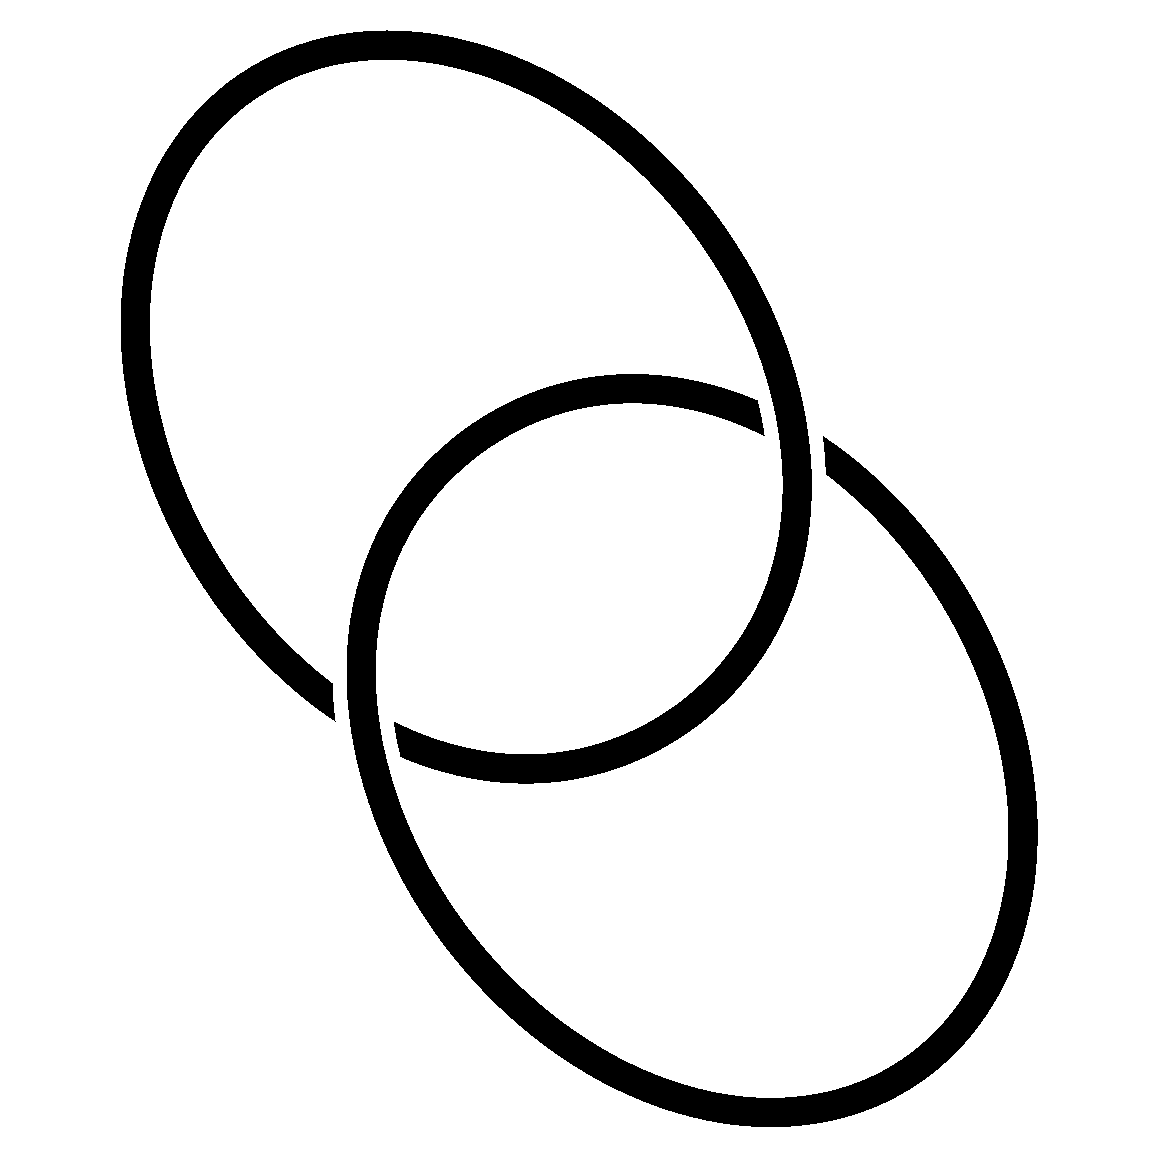
\includegraphics[width=2.5cm]{fig/2ringsd.eps}  &
      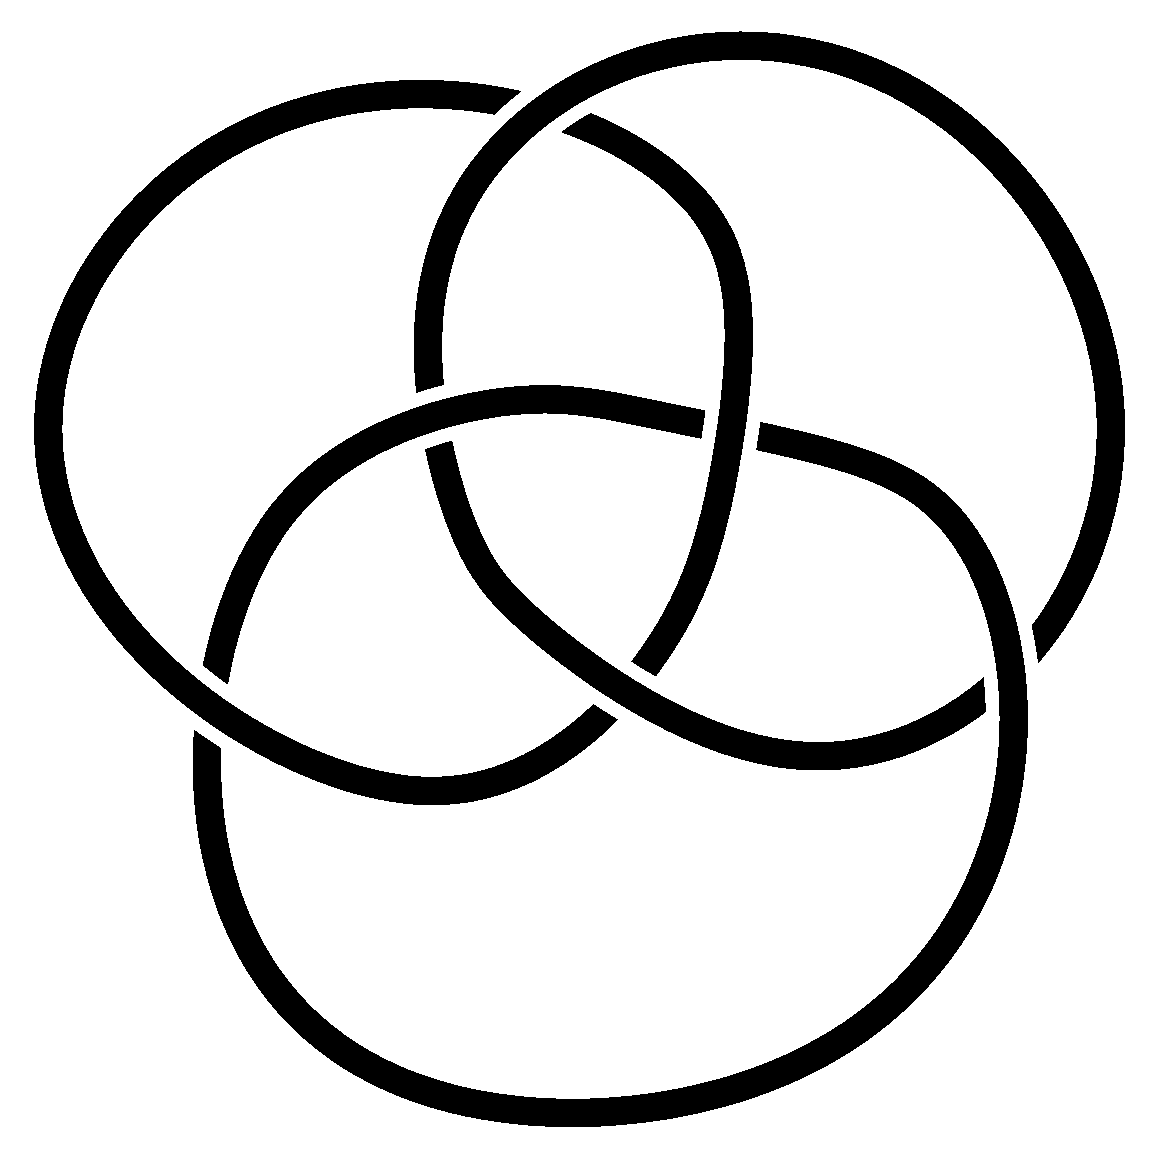
\includegraphics[width=2.5cm]{fig/borromeand.eps} \\
      (A) & (B) & (C) & (D) & (E) \\
\end{tabular}
   \end{center}
   \vspace{-0.7cm}
   \caption{ Knots and links diagrams}
   \label{fig:links3ddiagrams}
\end{figure}

So, a link diagram can be seen as a 4-regular {\it plane graph} with
an extra information on each vertex. For example, the trefoil may be
seen as the plane graph of Figure \ref{fig:linksDiagramElements}A.
The extra information of the vertices is shown on Figure
\ref{fig:linksDiagramElements}B and it encodes, in an intuitive way,
exactly the information of which ``cylinder segment'' is on top and
which ``cylinder segment'' is below. Note that there are two
possibilities for this ``extra information''. They are shown in
Figure~\ref{fig:linksDiagramElements}C. The $a$ curve ($b$ curve) in
this figure is said to be the {\it overcrossing} ({\it
undercrossing}) line in the top case and the {\it undercrossing}
({\it overcrossing}) line in the bottom case.

\begin{figure}[htp]
   \begin{center}
   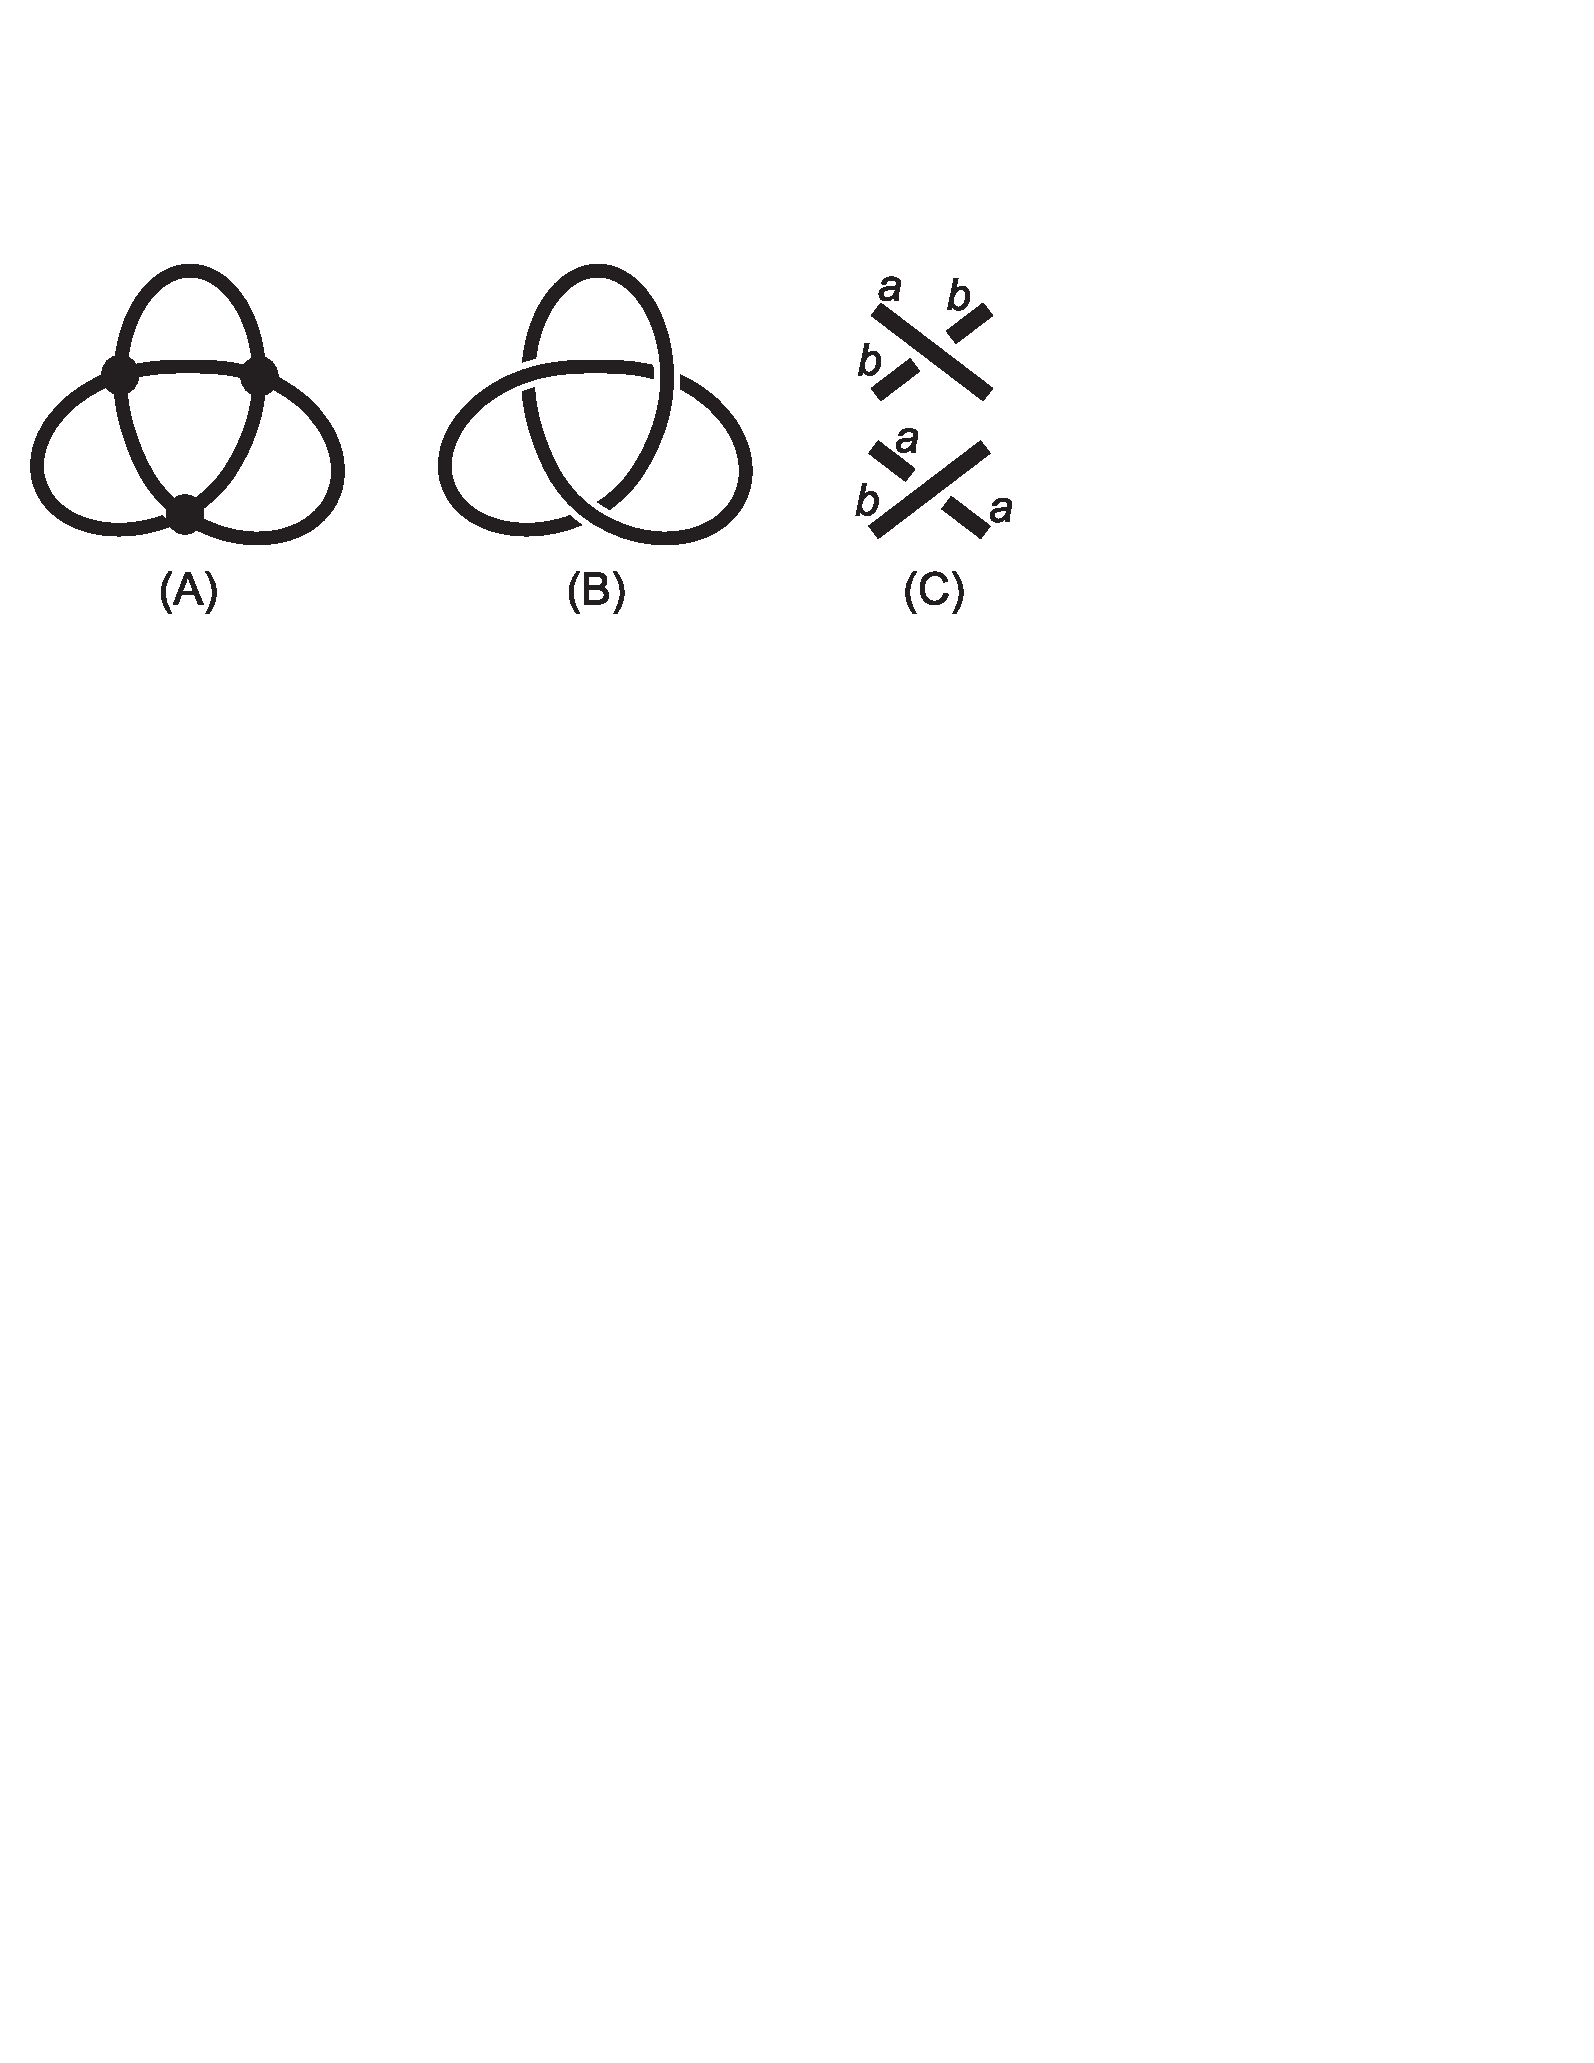
\includegraphics[width=10cm]{fig/linkDiagramElements.eps}
   \end{center}
   \vspace{-0.7cm}
   \caption{ Link diagram as plane graphs}
   \label{fig:linksDiagramElements}
\end{figure}

Given two links, an interesting question to answer is whether these
links can be aligned without tearing any of the strings. For example
the links $A$ and $B$ given by their diagrams on
Figure~\ref{fig:exampleOfAmbientIsotopicKnots} can be aligned as is
shown. Imagine this sequence of ``moves'' transforming $A$ and $B$
occurring on the 3-dimensional space. It is intuitive that we need
no tearing.
\begin{figure}[htp]
   \begin{center}
   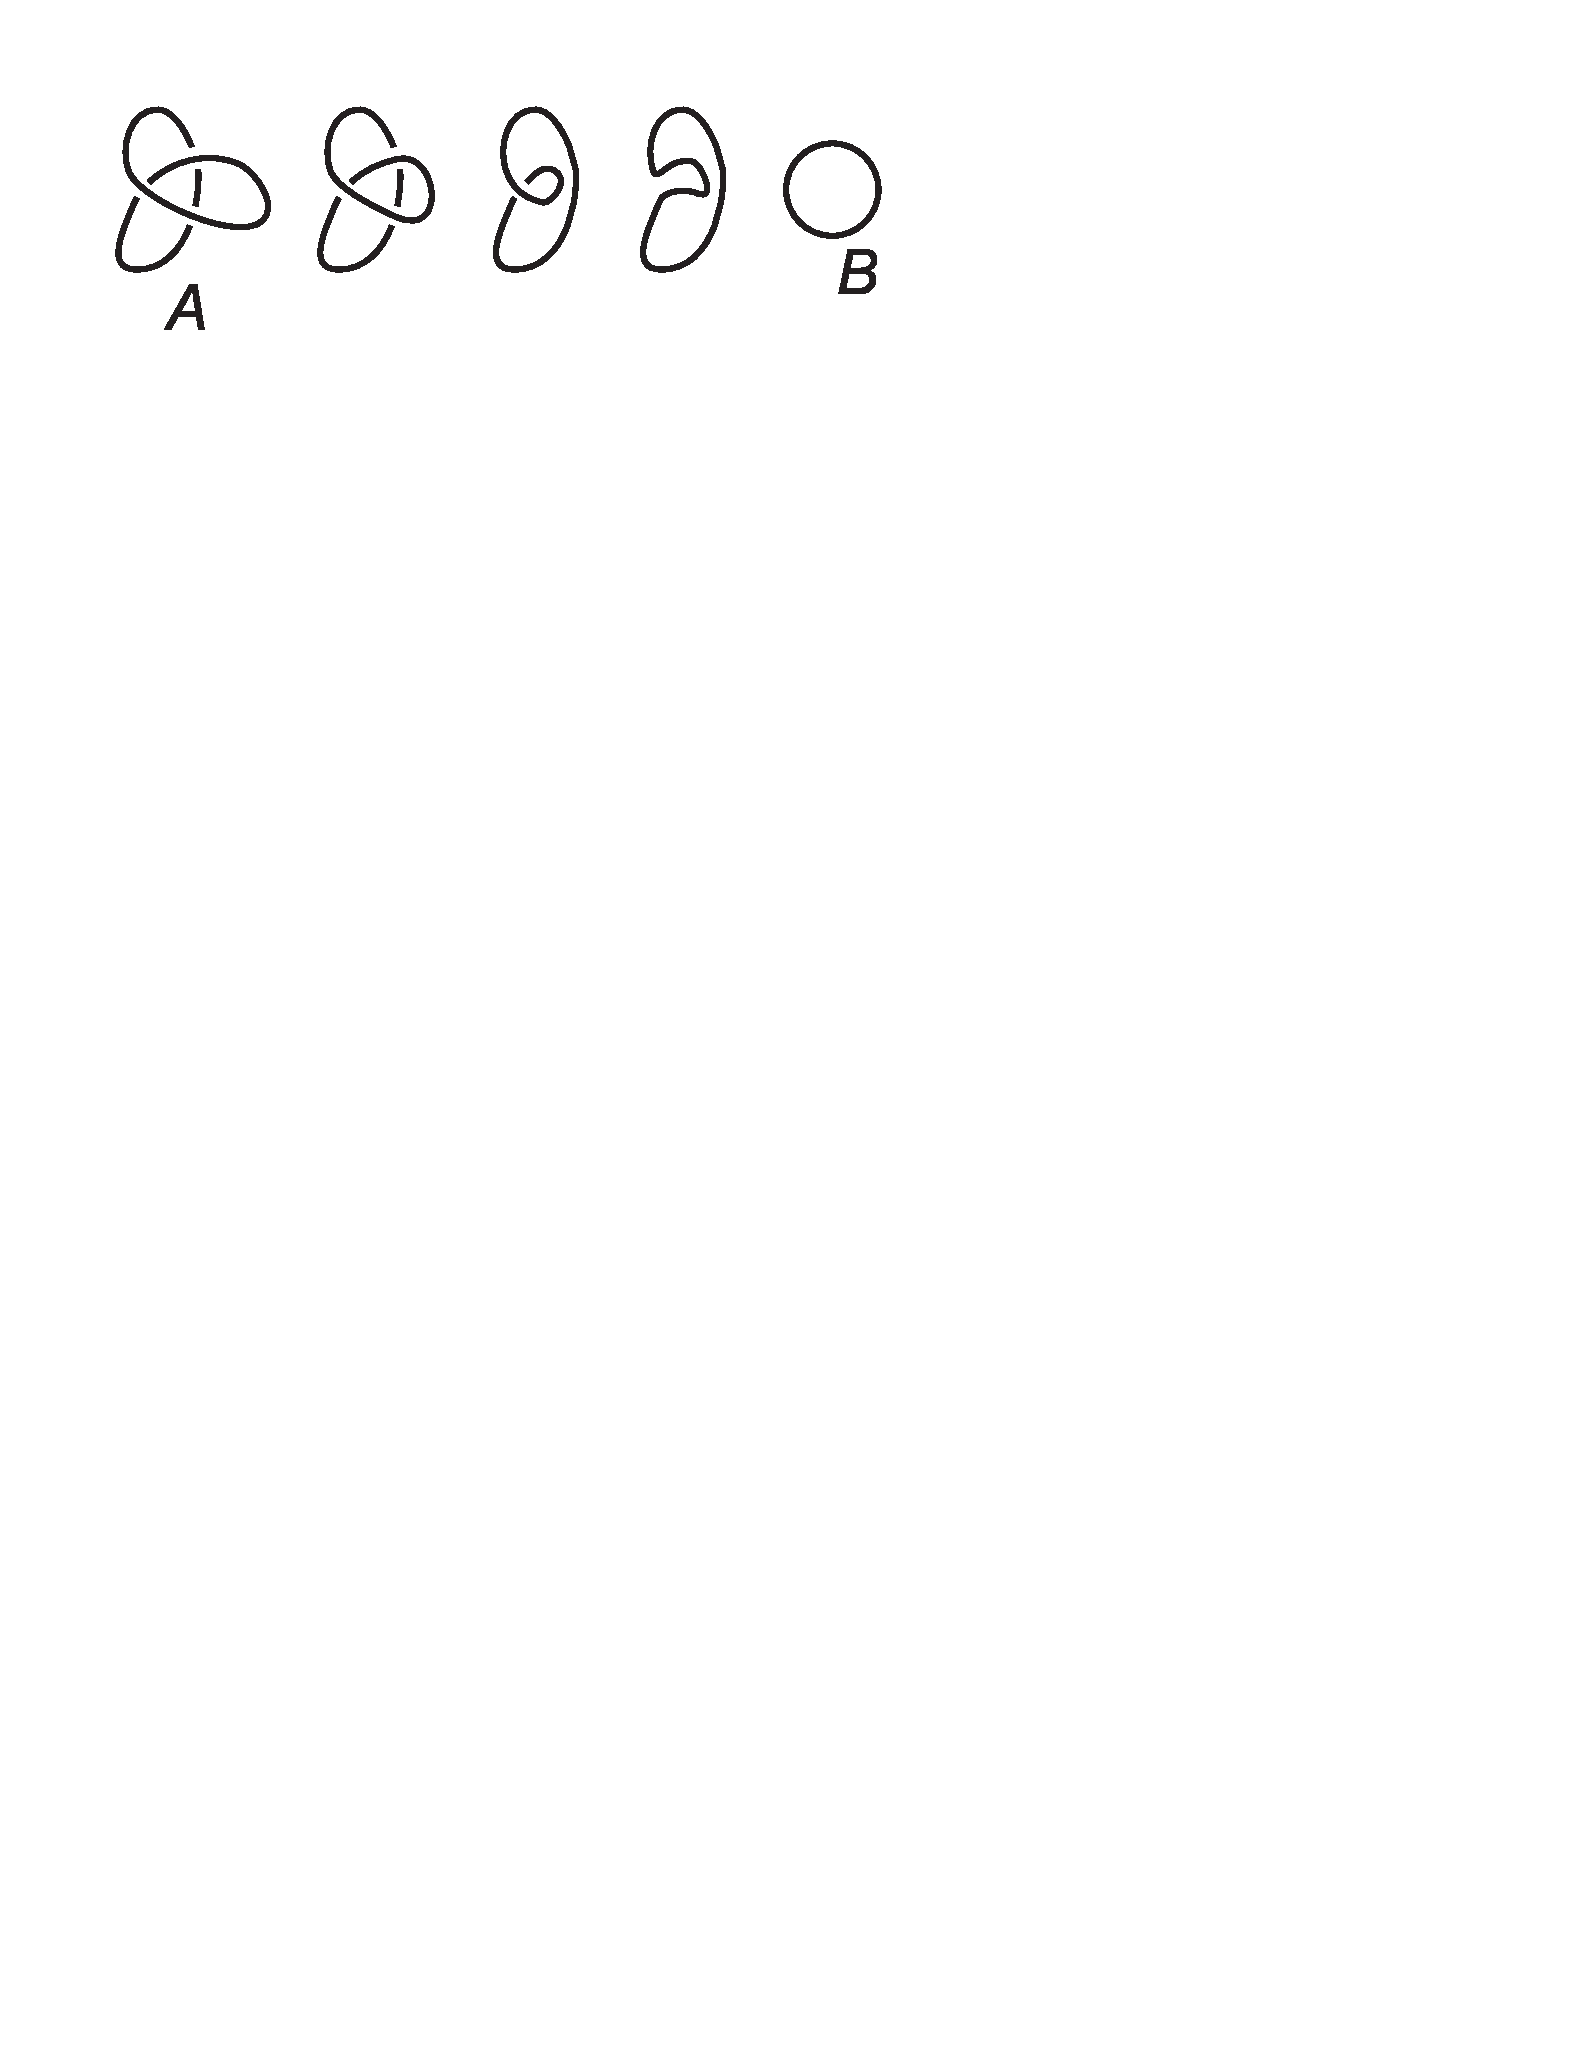
\includegraphics[width=10cm]{fig/exampleOfAmbientIsotopicKnots.eps}
   \end{center}
   \vspace{-0.7cm}
   \caption{ Ambient isotopic knots}
   \label{fig:exampleOfAmbientIsotopicKnots}
\end{figure}
On the other hand, the circle and the trefoil (note the crossings on
$A$ to see that it is not a trefoil) cannot be aligned without
tearing. These are examples of the placement problem for links. We
say two links are placed the same way in 3-dimensional space if this
alignment can be done. The formal term for this alignment, defined
in Section~\ref{sec:topology}, is: ambient isotopy. Ambient isotopy
is an equivalence relation and when we say that links are equivalent
we are referring to the ambient isotopy relation. So $A$ and $B$ in
Figure~\ref{fig:exampleOfAmbientIsotopicKnots} are equivalent, but
are not equivalent to the trefoil.
\begin{figure}[htp]
   \begin{center}
   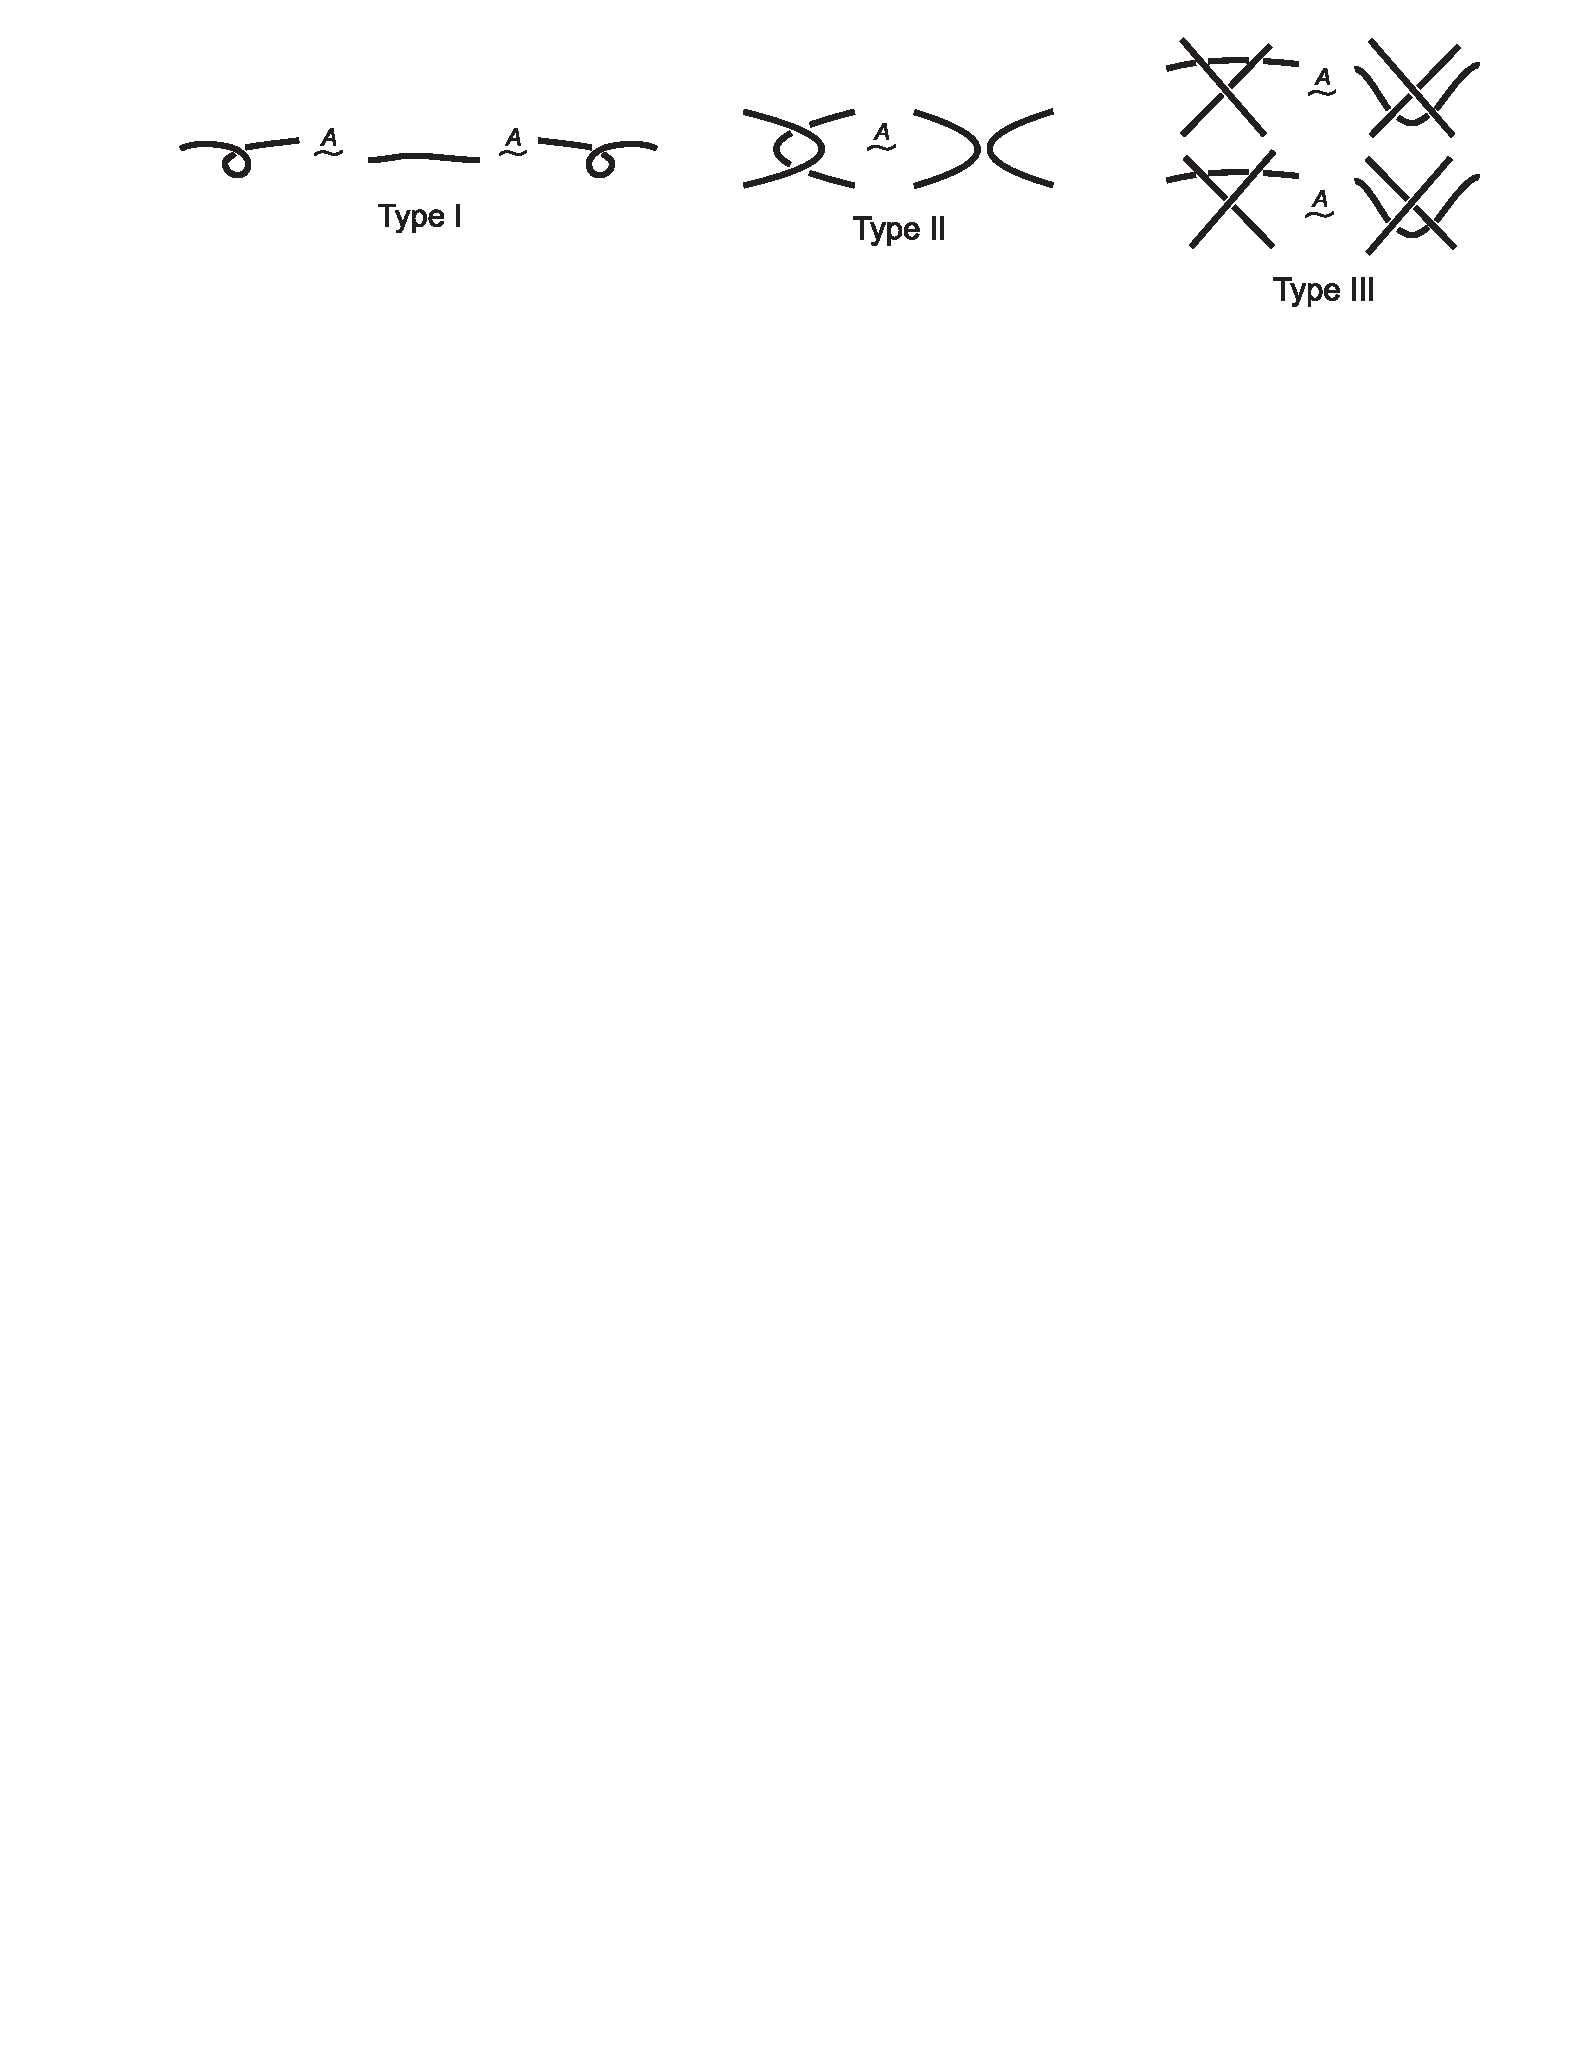
\includegraphics[width=15cm]{fig/ReidemeisterMoves.eps}
   \end{center}
   \vspace{-0.7cm}
   \caption{ Reidemeister moves}
   \label{fig:ReidemeisterMoves}
\end{figure}

Reidemeister \cite{Reidemeister1932} proved the following result
about link equivalence in the diagrammatic language:
\begin{center}\it two links are equivalent ({\it i.e.} ambient isotopic) if
and only if  \linebreak any diagram of one link can be transformed
into a diagram for the other link \linebreak  via a sequence of
Reidemeister Moves (Figure~\ref{fig:ReidemeisterMoves}).
\end{center}
We use the symbol $\Aequiv$ between two link diagrams or detached
pieces of link diagrams (where the boundaries of these pieces have a
correspondence that should be clear) to denote that they are ambient
isotopic. Note that the Reidemeister moves we used in the
transformation of Figure~\ref{fig:exampleOfAmbientIsotopicKnots}
were type II move, type I move and alignments. The three
Reidemeister moves will be also called $RE_1$, $RE_2$ and $RE_3$ for
moves of type I, type II and type III, respectively. Two link
diagrams that differ by a finite sequence of Reidemeister moves
$RE_2$ and $RE_3$ are said to be {\it regular isotopic}. The
notation $A \Requiv B$, where $A$ and $B$ are link diagrams, is used
to say that $A$ and $B$ are regular isotopic. Note that regular
isotopic diagrams are always ambient isotopic,
$$ A \Requiv B \implies A \Aequiv B,$$
while the converse is not always true. Observe that the regular
isotopic relation between link diagrams defines an equivalence
relation on the set of link diagrams. This relation is called {\it
regular isotopy}.

Link diagrams interpreted as  {\it blackboard framed links}, as we
will see later, is a presentation for spaces ({\it i.e.} connected,
compact, oriented 3-manifolds). This connection is
essential to the contribution of this work: a prime space catalog of
small BFLs or blinks.

\newpage

\section{Linking number, writhe and linking matrix}

A link is said {\it oriented} if all its components have an {\it
orientation}. There are two possible orientations for each
component. So, a link with $k$ components can be oriented in $2^k$
different ways. To present an oriented link we can draw the link
diagram with one arrow on each component indicating its orientation.
For example, Figure~\ref{fig:orientedLinks}A shows an oriented
trefoil. A crossing on an oriented link diagram may be of two types
as Figure~\ref{fig:orientedLinks}C shows. Each of these types has a
number +1 or -1 which is called the {\it sign of the (oriented)
crossing}. When the undercrossing line, on its orientation sees the
overcrossing line go from left to right then the sign is +1, else,
if it sees the overcrossing line going right to left, the sign is
-1.
\begin{figure}[htp]
   \begin{center}
   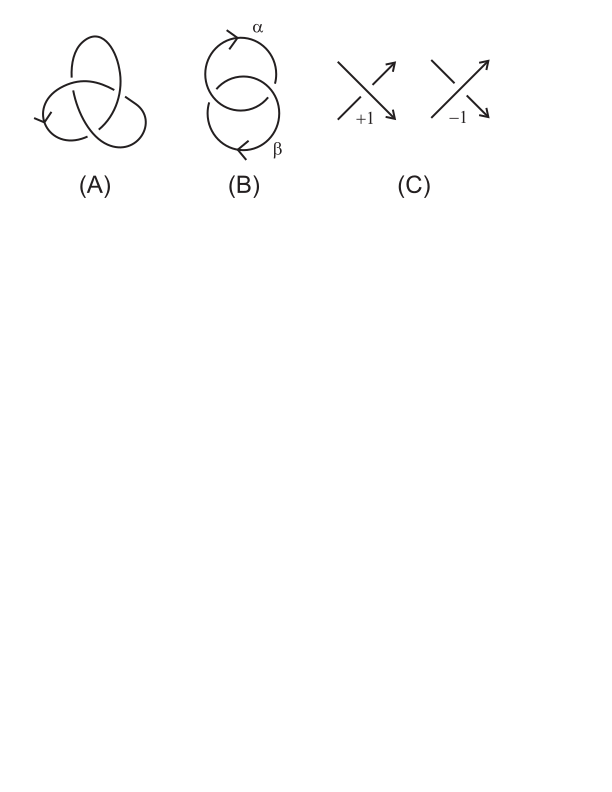
\includegraphics[width=9cm]{fig/orientedLinks.eps}
   \end{center}
   \vspace{-0.7cm}
   \caption{ Oriented links}
   \label{fig:orientedLinks}
\end{figure}

Let $D$ be an oriented link diagram of link $L$. Let $\alpha$ be a
component of $L$. The sum of the signs of auto-crossings of $\alpha$
(crossings of $\alpha$ with $\alpha$) on $D$ is said to be its {\it
writhe} and is denoted by $w(\alpha)$. For instance, the writhe of
the only component of the oriented trefoil of
Figure~\ref{fig:orientedLinks}A is +3, because all 3 crossing are
auto-crossings and with sign +1. Note that changing the orientation
of a component does not change its writhe. Now, let $\alpha$ and
$\beta$ be two components of a link $L$. The sum of the signs of the
crossings on $D$ of components $\alpha$ and $\beta$ is said to be
its {\it linking number} and is denoted by $\ell k(\alpha,\beta)$.
For instance, on Figure~\ref{fig:orientedLinks}B, the linking number
of $\alpha$ and $\beta$ is -2 as the two crossings are -1.

Let $D$ be an oriented link diagram with components $\alpha_1$,$\alpha_2$,$\ldots$,
$\alpha_n$. The {\it linking matrix} of $D$ is given by
$$\left(\begin{array}{cccc}
    w(\alpha_1) & \ell k(\alpha_1,\alpha2) & \cdots & \ell k(\alpha_1,\alpha_n) \\
    \ell k(\alpha_2,\alpha_1) & w(\alpha_2) & \cdots & \ell k(\alpha_2,\alpha_n) \\
    \vdots & \vdots & \ddots & \vdots \\
    \ell k(\alpha_n,\alpha_1) & \ell k(\alpha_n,\alpha_2) & \cdots & w(\alpha_n)
  \end{array}\right)
$$ From this matrix, as we will see in Section~\ref{sec:homologyGroup}, it is
possible to obtain a space invariant: the homology group. But to
understand this we must first understand what a link diagram has to
do with spaces. This is the theme of next section.

\section{Framed links and blackboard framed links: encoding spaces}
\label{sec:bfl}

This section presents a fundamental result for this work. To get
deep into this result's justification ideas would demand a lot of
work not needed for our aim. But to get a good image of this
result's meaning is easier. Let's get it.

Consider the unknot on $\IS^3$, {\it i.e.} a ring floating inside the
3-dimensional sphere. Now imagine a small tubular volume $T$,
centered on this unknot. In this situation one could ask: is there a
way to replace the interior of this tubular volume $T$ with
something different? Of course there is. We could replace $T$ by
``nothing'', leading to the ``shape'' of $\IS^3$ with a toroidal hole in it.
Although this is a correct thought, it is not what we are imagining
here. We would like to replace $T$ with something different, but not
leaving a hole. In this case, is there something different of
``replacing $T$ by $T$''? The answer is also yes \footnote{For
theory and examples of these replacements see \cite{Rolfsen1976}.}.
We can replace $T$ by another volume that fills in the hole and
leads to a closed 3-manifold different from $\IS^3$. In fact, this
idea generalizes.

Let's call a replacement like the one we mentioned above by {\it
surgery}. Think of a link on $\IS^3$ and a thin tubular volume $T_i$
centered on each of its components. By analogy with the simple
unknot case above, it is easy to note the possibility of obtaining
different closed 3-manifolds by different surgeries ({\it i.e.}
replacement of the thin tubular volumes $T_i$). In fact, as
Lickorish \cite{Lickorish1962} and Wallace \cite{Wallace1960} proved
independently, any closed, connected, oriented 3-manifold may be
obtained by surgeries (the technical name is Denn surgeries) of a
link on $\IS^3$. So, by doing valid replacements of the thin tubular
volumes centered on the components of a link, one can obtain any
closed, connected, oriented 3-manifold. This result is very
important once shows an intrinsic connection between links ({\it
i.e.} embeddings of circles into the 3-dimensional sphere $\IS^1
\rightarrow \IS^3$) with spaces ({\it i.e.} closed, connected,
oriented 3-manifold).

The information that defines how to do the surgery on a component
(replacement of the tubular volume centered on that component) is
called {\it framing}. So, with a link and a framing for each of its
component, a space is defined. A framing as is justified in Chapter
9 of \cite{Rolfsen1976} may be just an integer number. This leads to
the definition we use of {\it framed link}: a link in $\IS^3$ with an
integer associated to each component. So, from a framed link it is
possible to obtain a space. Start with the link, define the thin
tubular volumes $T_i$ centered on each component and, finally, apply
the surgery on each $T_i$ defined by the framing of component $i$.

In Section~\ref{sec:knotsAndLinks} we saw that a link diagram is a
way to present a link. So, we can present framed links (spaces) by
drawing a link diagram and writing an integer near each component:
its framing. Although this is a nice way to present spaces, there is
an even more concise way to do it based on two facts: (1) the writhe
of a component, as is the framing of a component on a framed link,
is an integer number associated to it on a link diagram; (2) by
adding or removing one curl on a link diagram, application of one
Reidemeister move I, one is able to, without modifying the link,
increment by 1 or -1 the writhe of a component. Using these ideas we
have the following result:
\begin{center}
\it given any framed link, it is possible to draw a link
diagram\linebreak
 for it where the writhe of each component on the link diagram \linebreak
is exactly the framing of the same component.
\end{center}
For example, suppose we want a link diagram for the trefoil with
framing zero. See Figure~\ref{fig:blackboardFramedLink}. We first
draw a link diagram for the trefoil. While the framing of the
component is not equal to its writhe on the diagram, we add curls
until they match. Note that adding these curls do not change the
underlying link.
\begin{figure}[htp]
   \begin{center}
   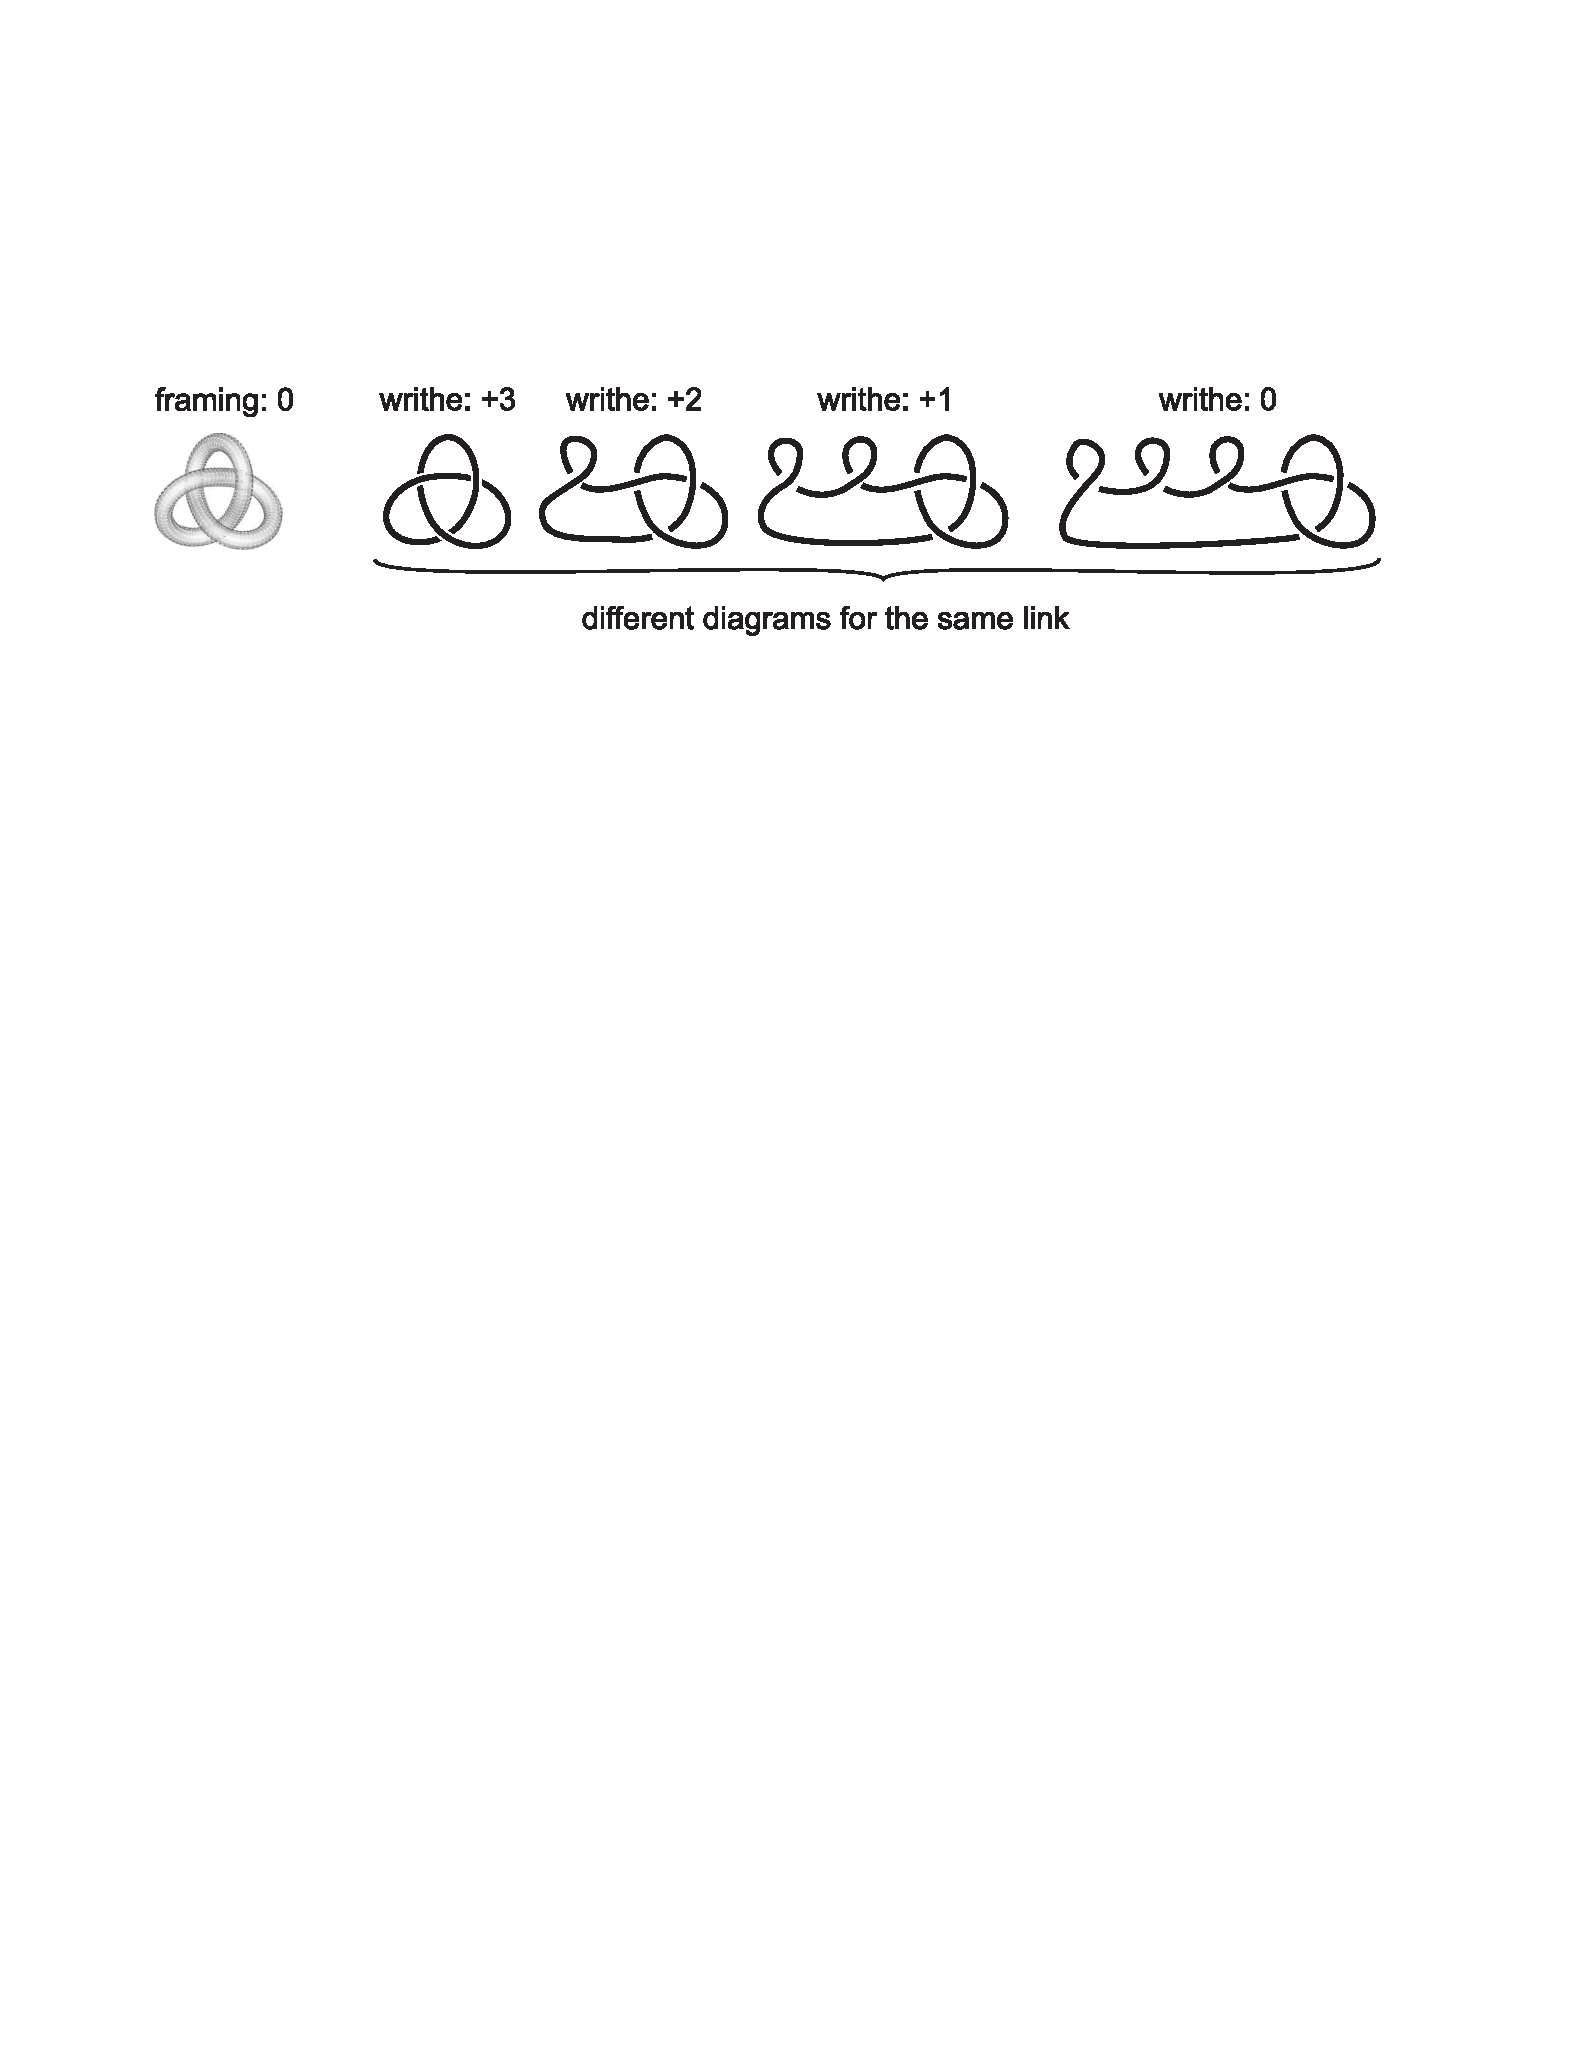
\includegraphics[width=12cm]{fig/blackboardFramedLink.eps}
   \end{center}
   \vspace{-0.7cm}
   \caption{ Aligning framing with writhe}
   \label{fig:blackboardFramedLink}
\end{figure}

A {\it blackboard framed link} or {\it BFL} is a link diagram
presentation of a space. The space is the space induced by a framed
link defined by: (1) the link of the framed link is the link on the
diagram; (2) the framing of each component equals to the writhe of
the same component on the diagram. So, any link diagram may be seen
as a blackboard framed link inducing a space and, also, any space
has blackboard framed link presentation for it. One of the main
aims of this work is to identify all prime spaces that have a
``small blackboard framed link'' inducing it. 

\bigskip
\bigskip
\centerline{\large \textsc{How to fill the toroidal holes?}}
\bigskip

As we said, the framing tells how to close a toroidal 
hole in $\IS^3$. But how is that done? Here is how. 
A hole is a solid torus embedded in $\IS^3$. 
If the framing in zero, then define $c$ as a curve on the surface of the hole
(\ie a solid torus)  
parallel to the curve that follows the center of 
the hole (see the black line in the left drawing of
Figure~\ref{fig:unknotWithMeridian}). If the framing 
is $n \neq 0$ then define $c$ the same way except 
that it does $n$ twists on the surface of the hole 
before completing a loop (see the bottom drawing 
in Figure~\ref{fig:unknotWithMeridian}). To close the 
toroidal hole is a matter of doing an abstract gluing:
identify curve $c$ with the meridian curve of a torus 
as is shown by the ``glue'' arrow in 
Figure~\ref{fig:unknotWithMeridian}. With this 
identification a complete homeomorphism is defined 
between ``the hole'' and ``the shape'' that replaces 
it in a different way.


%Each component of a
%BFL is ``over''
%\footnote {it never crosses (not even touches) the
%intersection the projection of boundary of the whole into our
%reference plane}
%the surface  of a toroidal hole in $\IS^3$ which is
%closed by a solid torus so that the component and the meridian curve
%of the solid torus become the same, see Figure
%\ref{fig:unknotWithMeridian}.

\begin{figure}[htp]
   \begin{center}
   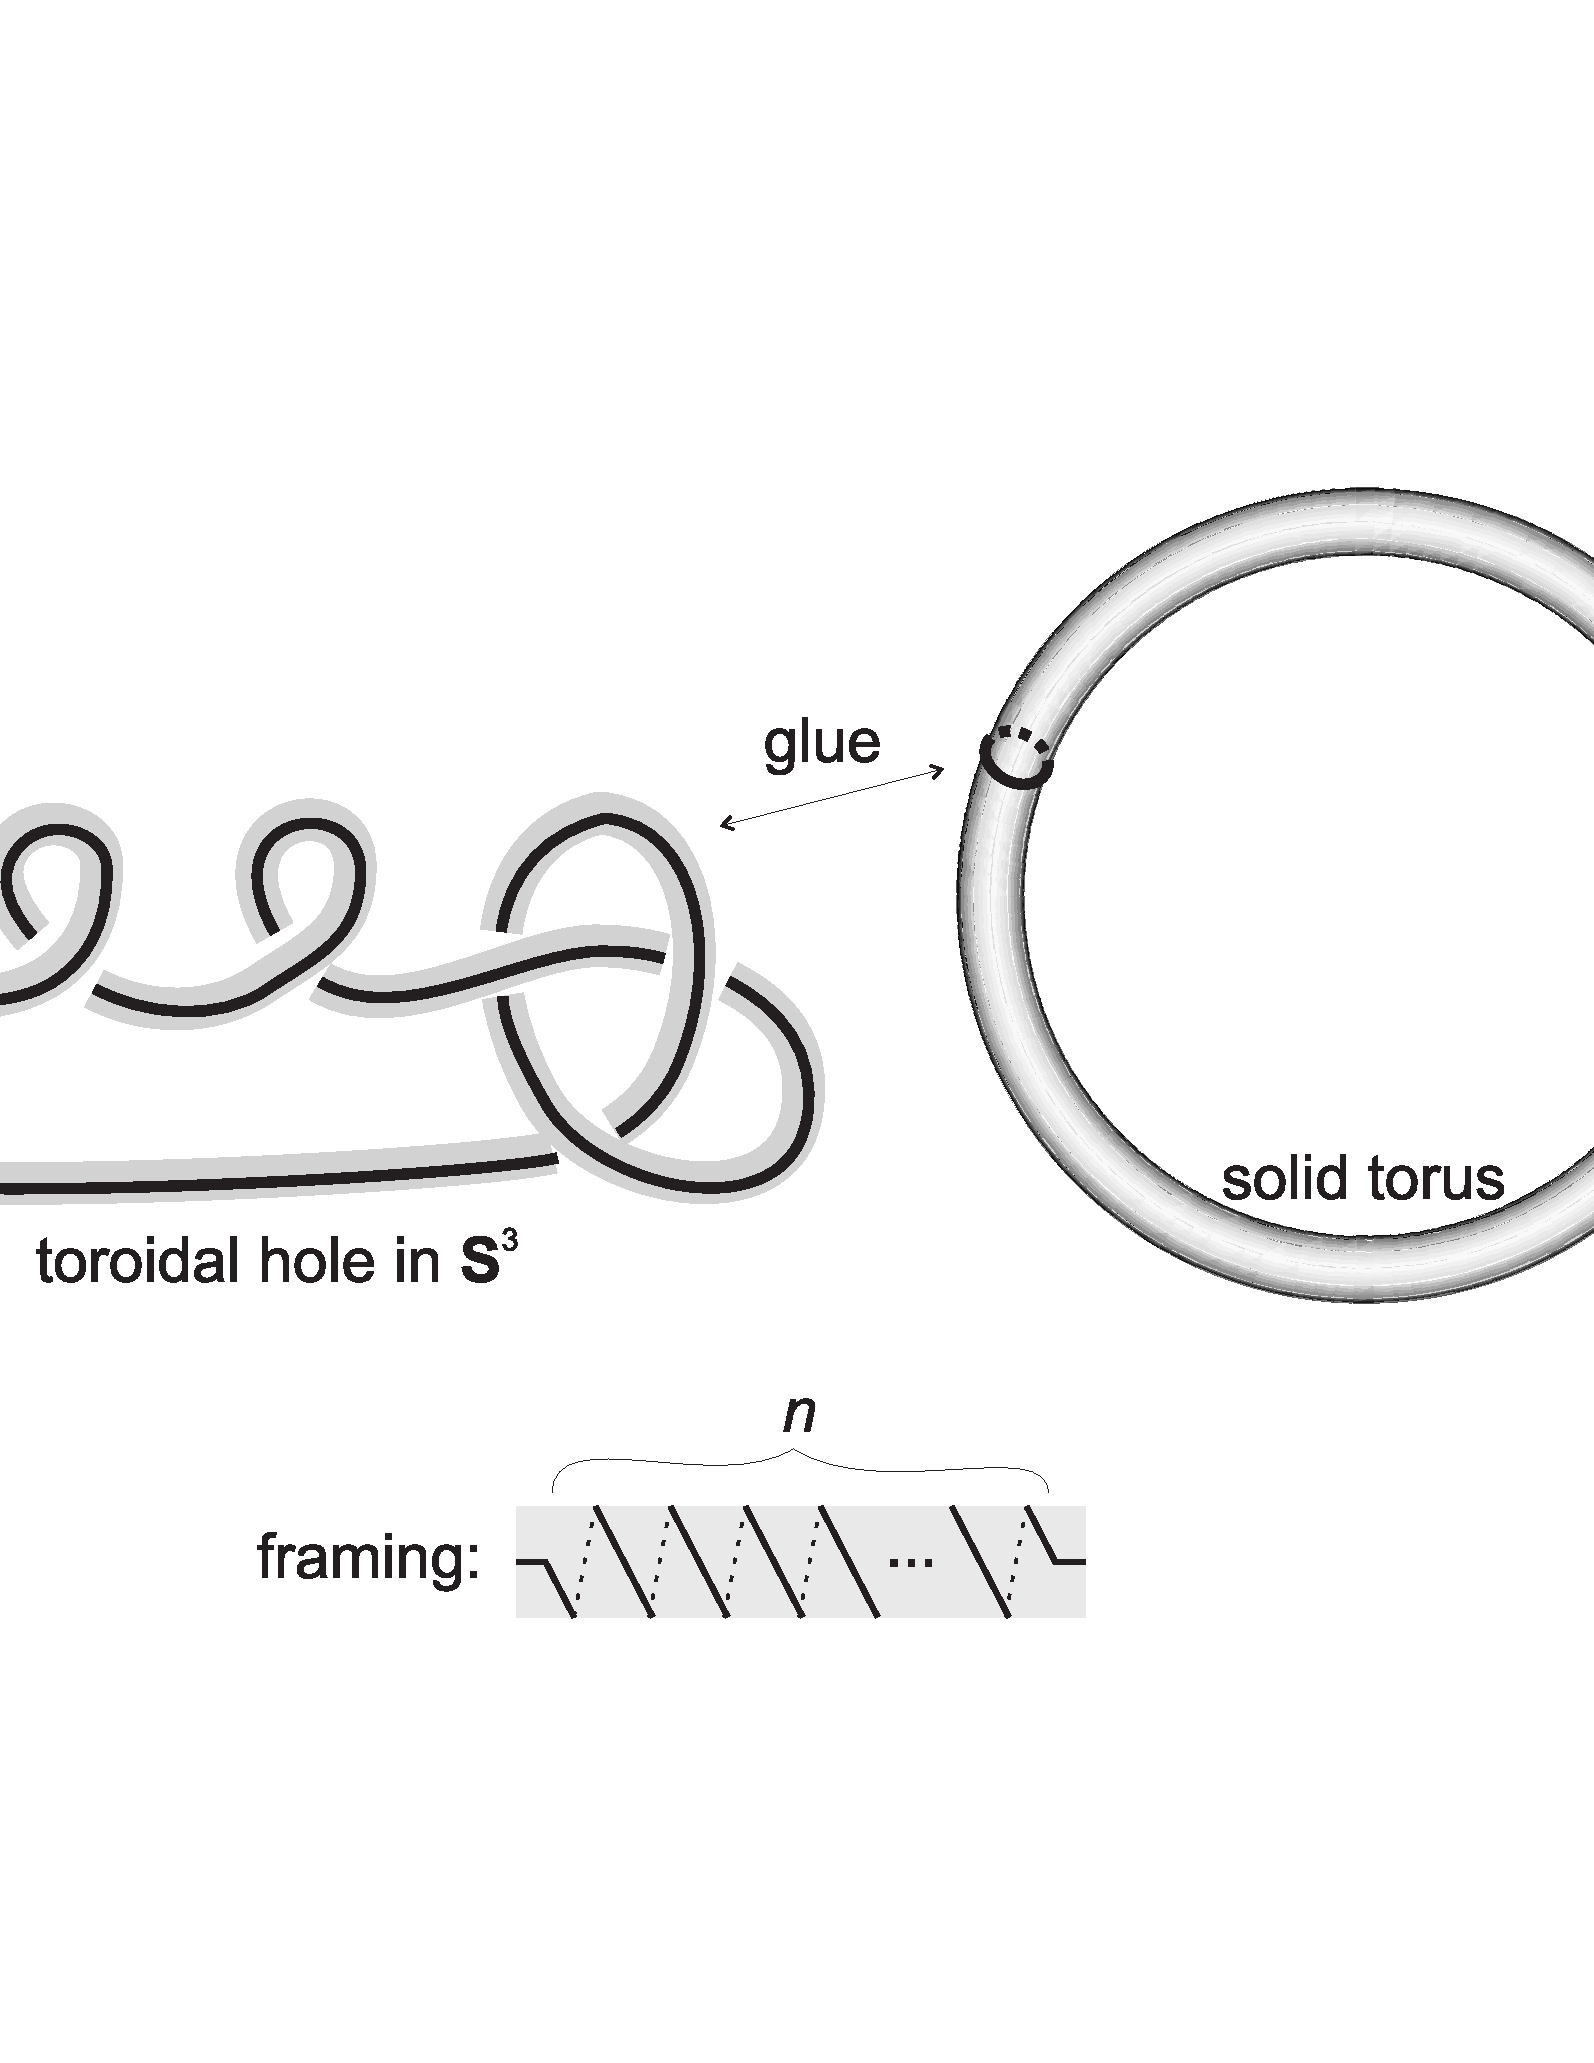
\includegraphics[width=7cm]{fig/unknotWithMeridian.eps}
   \end{center}
   \vspace{-0.7cm}
   \caption{ Gluing a solid torus
   to a toroidal hole: BFL-component and meridian become the same}
   \label{fig:unknotWithMeridian}
\end{figure}


\begin{comment}
For example, let $T'$ be a volume exactly equal to $T$. There of the
boundary of $T$ to is an homeomorphism that it is possible to
replace $T$ by $T'$ as shown in Figure~\ref{fig:surgery}, by
defining an homeomorphism between the boundaries of $T$ and $T'$
such that a meridian on $T$ is mapped to a longitude line. This
fills the hole and leads to a connected, compact, oriented
3-manifold different from $\IS^3$.

\begin{figure}[htp]
   \begin{center}
   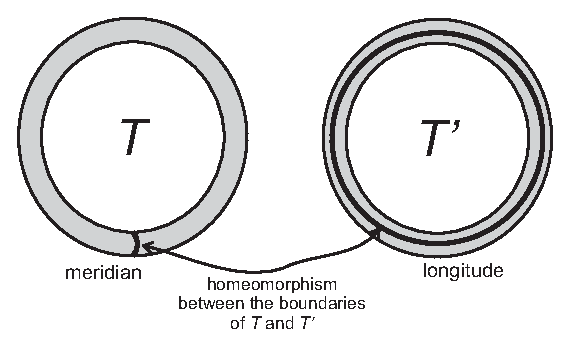
\includegraphics[width=9cm]{fig/surgery.eps}
   \end{center}
   \vspace{-0.7cm}
   \caption{ Oriented links}
   \label{fig:surgery}
\end{figure}


{\red Linking Number, Writhe} Any framed link with integral framing
on its components can be encoded as a link diagram that, in this
case, is called a {\em blackboard framed link} or {\em BFL}. As is
known {\color{red} (cite this result)}, any space has a framed link
with integral framing on each component that induces it. A
consequence of these facts is that any space also has a blackboard
framed link inducing it. To summarize, a blackboard framed link is a
space presented as a link diagram.

\end{comment}

\newpage

\section{A calculus on blackboard framed links}
\label{sec:BFLcalculus}

When do two framed links induce the same space? Kirby, in
\cite{Kirby1978}, showed when. Fenn and Rourke
\cite{FennAndRourke1979} reformulated Kirby's ideas, and, from that
point, Kauffman brought Kirby's result to the diagrammatic language
of blackboard framed links. Figure~\ref{fig:kauffmancalculus} shows
Kauffman's blackboard framed link formulation of Kirby's calculus
(page 260 of \cite{Kauffman1991}).
\begin{figure}[htp]
   \begin{center}
      \leavevmode
      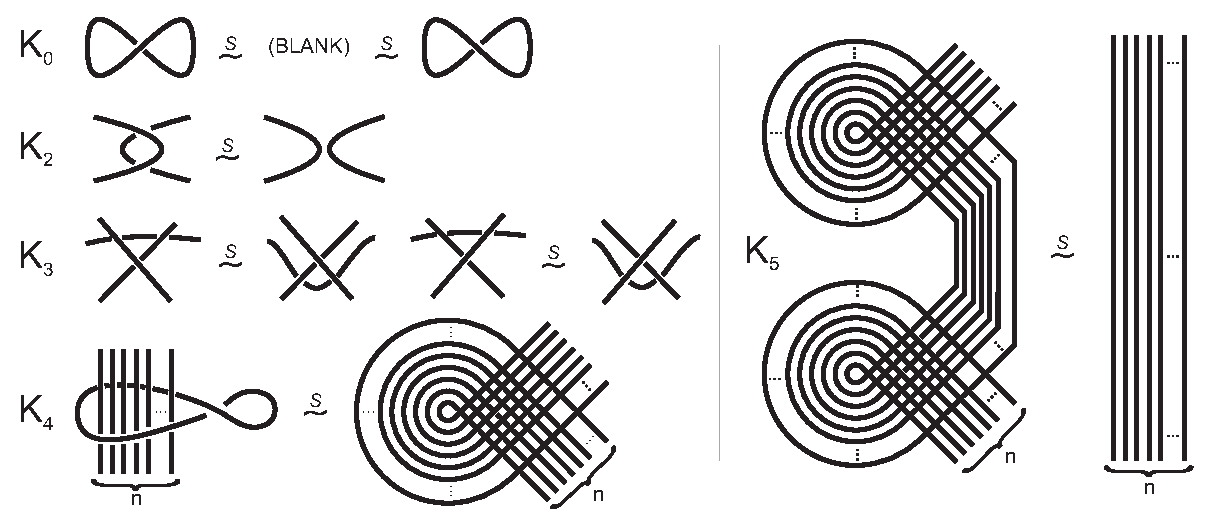
\includegraphics[width=15cm]{fig/kauffmancalculus.eps}
   \end{center}
   \vspace{-0.7cm}
   \caption{ Kauffman's blackboard framed link formulation of Kirby's
   calculus}
   \label{fig:kauffmancalculus}
\end{figure}

Some notes about Figure~\ref{fig:kauffmancalculus}. The symbol
$\Sequiv$ between two blackboard framed links denotes that both BFLs
induce the same space. When the symbol $\Sequiv$ is used between two
detached pieces of blackboard framed links (the correspondence on
the boundary of these pieces must exist and should be easily
identifiable as in Figure~\ref{fig:kauffmancalculus}) it means that
exchanging these pieces on any blackboard framed link do not change
the induced space. Move $K_0$ states that we can create or eliminate
disjoint knots in form of $\infty$ as we wish, that the induced
space does not change. Note that there is no $K_1$. We reserved this
label for a move shown later. Moves $K_2$ and $K_3$ are,
respectively, Reidemeister moves $RE_2$ and $RE_3$. So, regular
isotopic blackboard framed links (this relation is also defined for
BFL, once BFLs are link diagrams) induce the same space,
$$A \Requiv B \implies A \Sequiv B,$$
because there is a finite sequence of moves in $\{K_2, K_3\}$
connecting them. Moves $K_4$ and $K_5$ are actually a family of
infinite moves indexed by a parameter $n \in \IN$.

Kauffman's reformulation of Kirby's result states
that
\vspace{-0.2cm}
\begin{center} \it
 if $A$ and $B$ are blackboard framed links, then $A$ and $B$ induce the same
 space \linebreak
 if and only if applying a finite sequence of moves in $\{K_0, K_2, K_3, K_4(n),
 K_5(n)\}$ \linebreak
 one can transform $A$ into $B$.
\end{center}
As an application of this result, see
Figure~\ref{fig:exampleBFLCalculus}. All drawings are
blackboard framed link versions of the same space as they are all
connected by a finite sequence of moves in  $\{K_0, K_2, K_3,
K_4(n), K_5(n)\}$. One can verify, by applying the surgeries on
$\IS^3$ defined by each of these BFL's, that the resulting space is
$\IS^2 \times \IS^1$ (See \cite{Rolfsen1976}).
\begin{figure}[htp]
   \begin{center}
      \leavevmode
      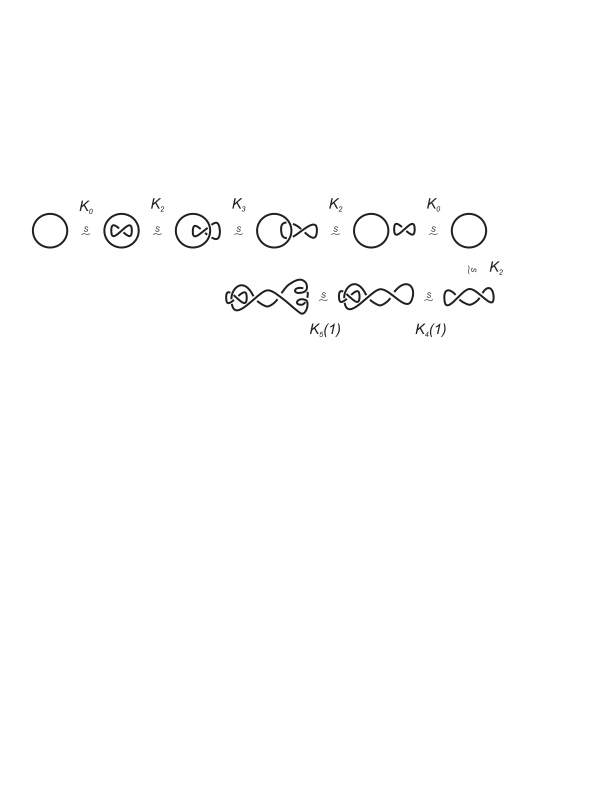
\includegraphics[width=13cm]{fig/exampleBFLCalculus.eps}
   \end{center}
   \vspace{-0.7cm}
   \caption{ Example of BFL's inducing the same
   space: $\IS^2 \times \IS^1$}
   \label{fig:exampleBFLCalculus}
\end{figure}

We denote by ${\cal K}^0$ Kauffman's set of moves or axioms on
Figure~\ref{fig:kauffmancalculus}: $${\cal K}^0 = \{ K_0, K_2, K_3,
K_4(n), K_5(n) \}.$$ We reserve the remainder of this section to
show that the move defined on Figure~\ref{fig:ribbonMove}, called
the {\it ribbon move}, and denoted by $K_1$, can replace the
infinite class of moves $K_5(n)$ on ${\cal K}^0$ leading to a
simpler and equivalent calculus ${\cal K}^1$.
\begin{figure}[htp]
   \begin{center}
      \leavevmode
      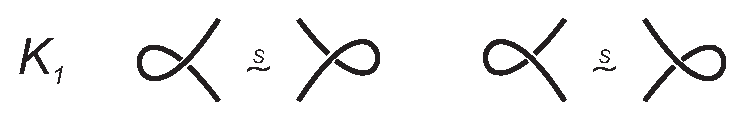
\includegraphics[width=8.5cm]{fig/ribbonmove.eps}
   \end{center}
   \vspace{-0.7cm}
   \caption{ The {\it ribbon move} or $K_1$}
   \label{fig:ribbonMove}
\end{figure}
Let's start by showing that the ribbon~move is a consequence of
${\cal K}^0$. But, before, we need a simple lemma.

\begin{Lem}[Whitney trick] Blackboard framed links that differ by
the pieces below are regular isotopic, so they induce the same
space.
\begin{center}
      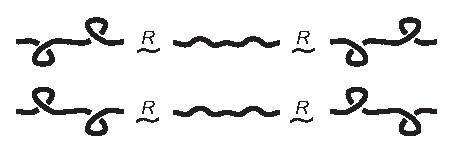
\includegraphics[width=8cm]{fig/whitneytrickresult.eps}
\end{center}
 \label{lem:whitneytrick}
\end{Lem}

\vspace{-0.6cm}

\begin{proof} The four forms of this lemma are
obtained by combined reflections on the $x$ and $y$ axis of
transformation
\begin{center}
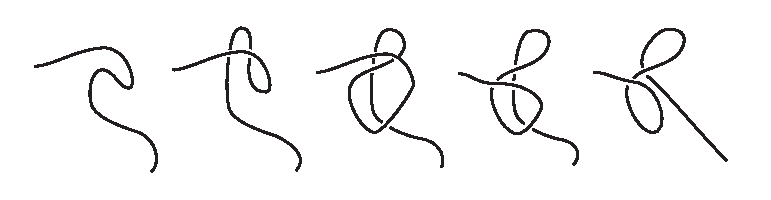
\includegraphics[width=12cm]{fig/whitneytrickproof.eps}.
\end{center}
Note that each passage is a regular isotopy move in $\{K_2, K_3\}$.
\end{proof}

\begin{Prop} The ribbon move follows from ${\cal K}^0$. More
specifically, from Whitney trick and the $n=1$ version of axiom
$K_5$.
\end{Prop}

\begin{proof} The following picture speaks by itself.
\begin{center}
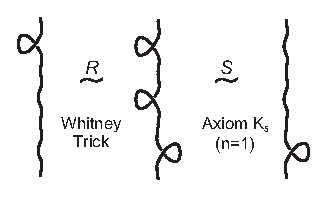
\includegraphics{fig/ribbonmoveproof.eps}
\end{center}
\vspace{-0.8cm}
\end{proof}

To show that $K_1$ actually can replace $K_5(n)$ it remains to prove
that with the remaining moves and $K_1$ ({\it i.e.} moves in$({\cal
K}^0 \backslash \{K_5(n)\}) \cup \{K_1\})$, we can reproduce
$K_5(n)$, for any $n$. Before doing this, we define some notation
and show some necessary results.

\begin{figure}[htp]
   \begin{center}
      \leavevmode
      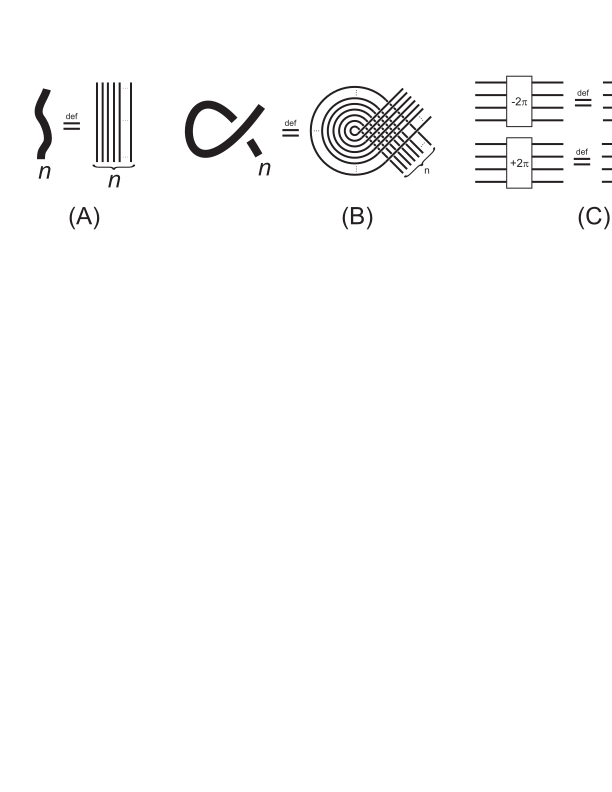
\includegraphics[width=13cm]{fig/someNotation.eps}
   \end{center}
   \vspace{-0.7cm}
   \caption{ Some notation}
   \label{fig:someNotation}
\end{figure}

Figure~\ref{fig:someNotation}A shows a thick cable with an $n$ near
it. This notation is a shortcut for $n$ parallel thin lines (the
ones we have been using). Figure~\ref{fig:someNotation}B shows a
thick cable with an $n$ near it doing a curl. This notation is a
shortcut for $n$ parallel lines doing a curl and respecting the
crossings as is shown. When a thicker cable appears without an $n$
and thin cables appear on the same link diagram, the $n$ is implicit
for the thicker cable. Figure~\ref{fig:someNotation}C shows the
definition of a {\em $+2\pi$ twist box} and of a {\em $-2\pi$ twist
box} both with {\em size} equals 4 (number of ``inputs''). The
extension of this definition for any size $\geq 2$ is immediate.

Now we show the last result before proving that $K_1$ may replace
$K_5(n)$. This result uses the $\pm2\pi$ twist boxes notation that
we defined earlier.

\begin{Lem} Regular isotopy leads to
\begin{center}
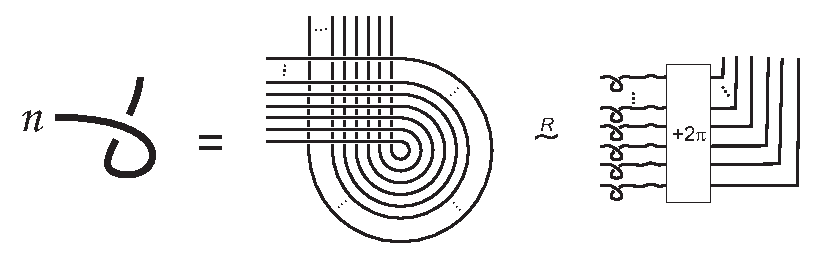
\includegraphics{fig/ncurland2pibox.eps}
\end{center}
\end{Lem}
\begin{proof}
Generalization of the following case where $n = 3$.
\begin{center}
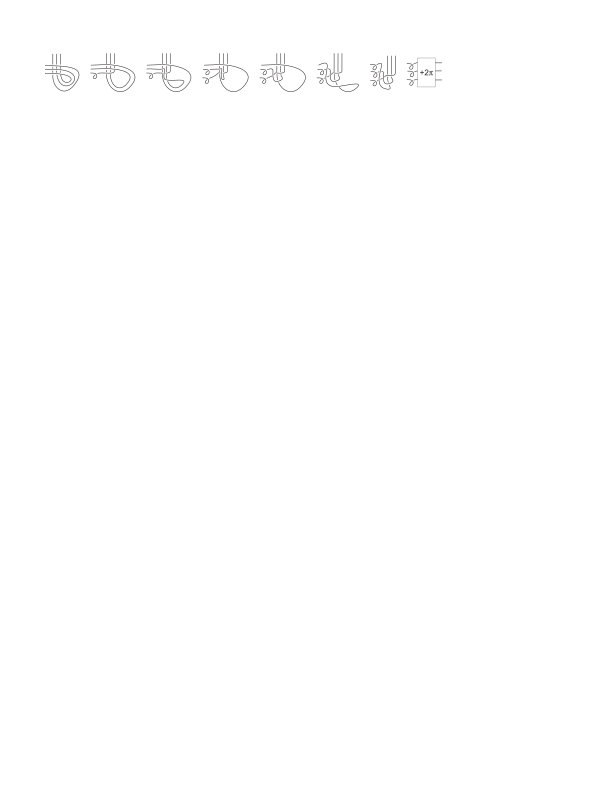
\includegraphics[width=15cm]{fig/ncurland2piboxProof2.eps}
\end{center}
\vspace{-0.8cm}
\end{proof}


\begin{Lem} Regular isotopy alone is capable of simplifying the left
configuration below with $2i^2$ crossings down to the right one with $2i$
crossings. \label{lem:istranistrands}
\begin{center}
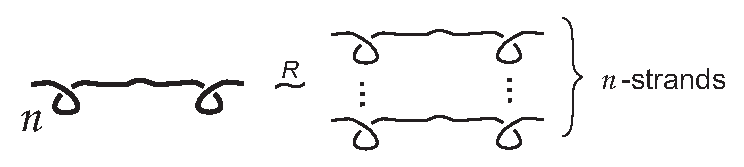
\includegraphics[width=9cm]{fig/istrandistrands.eps}
\end{center}
\end{Lem}
\begin{proof}
This proof is taken from \cite{Kauffman1991}.
\begin{center}
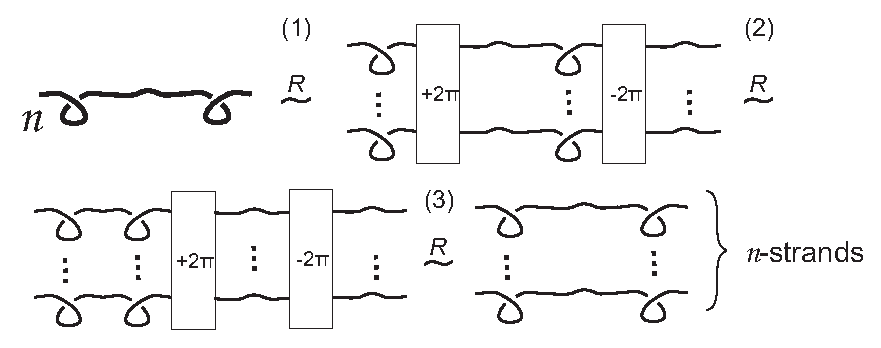
\includegraphics[width=10cm]{fig/istrandistrandsproof.eps}
\end{center}

\vspace{-1cm}
\end{proof}

\begin{Theo} The ribbon move $K_1$ together with regular isotopy
moves $K_2$ and $K_3$ implies move $K_5(n)$.
\end{Theo}

\vspace{-0.3cm}
\begin{proof} Follow this text and the figure below. We begin with
the left side of $K_5$ move. The passage (1) is the application of
Lemma \ref{lem:istranistrands}. The passage number (2) is the
application of ribbon moves on the bottom curl of each strand. The
passage number (3) is the application of Lemma
\ref{lem:whitneytrick} (Whitney trick) on each strand. The rightmost
image is the right side of move $K_5$, so the theorem is proved.
\begin{center}
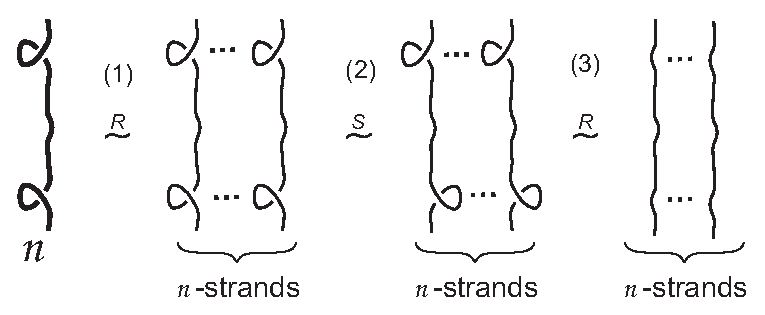
\includegraphics[width=9cm]{fig/ribbonmoveimpliesk5proof.eps}
\end{center}

\vspace{-1cm}
\end{proof}


Now we present Figure~\ref{fig:BFLcalculusK1} that shows
together all moves of ${\cal K}^1$ calculus: $${\cal K}^1 = \{ K_0, K_1, K_2, K_3, K_4(n)
\}.$$ Two BFLs induce the same space if and only if there is a
finite sequence of moves in $\{ K_0, K_1, K_2, K_3, K_4(n) \}$
transforming one BFL into the other.

\begin{figure}[htp]
   \begin{center}
      \leavevmode
      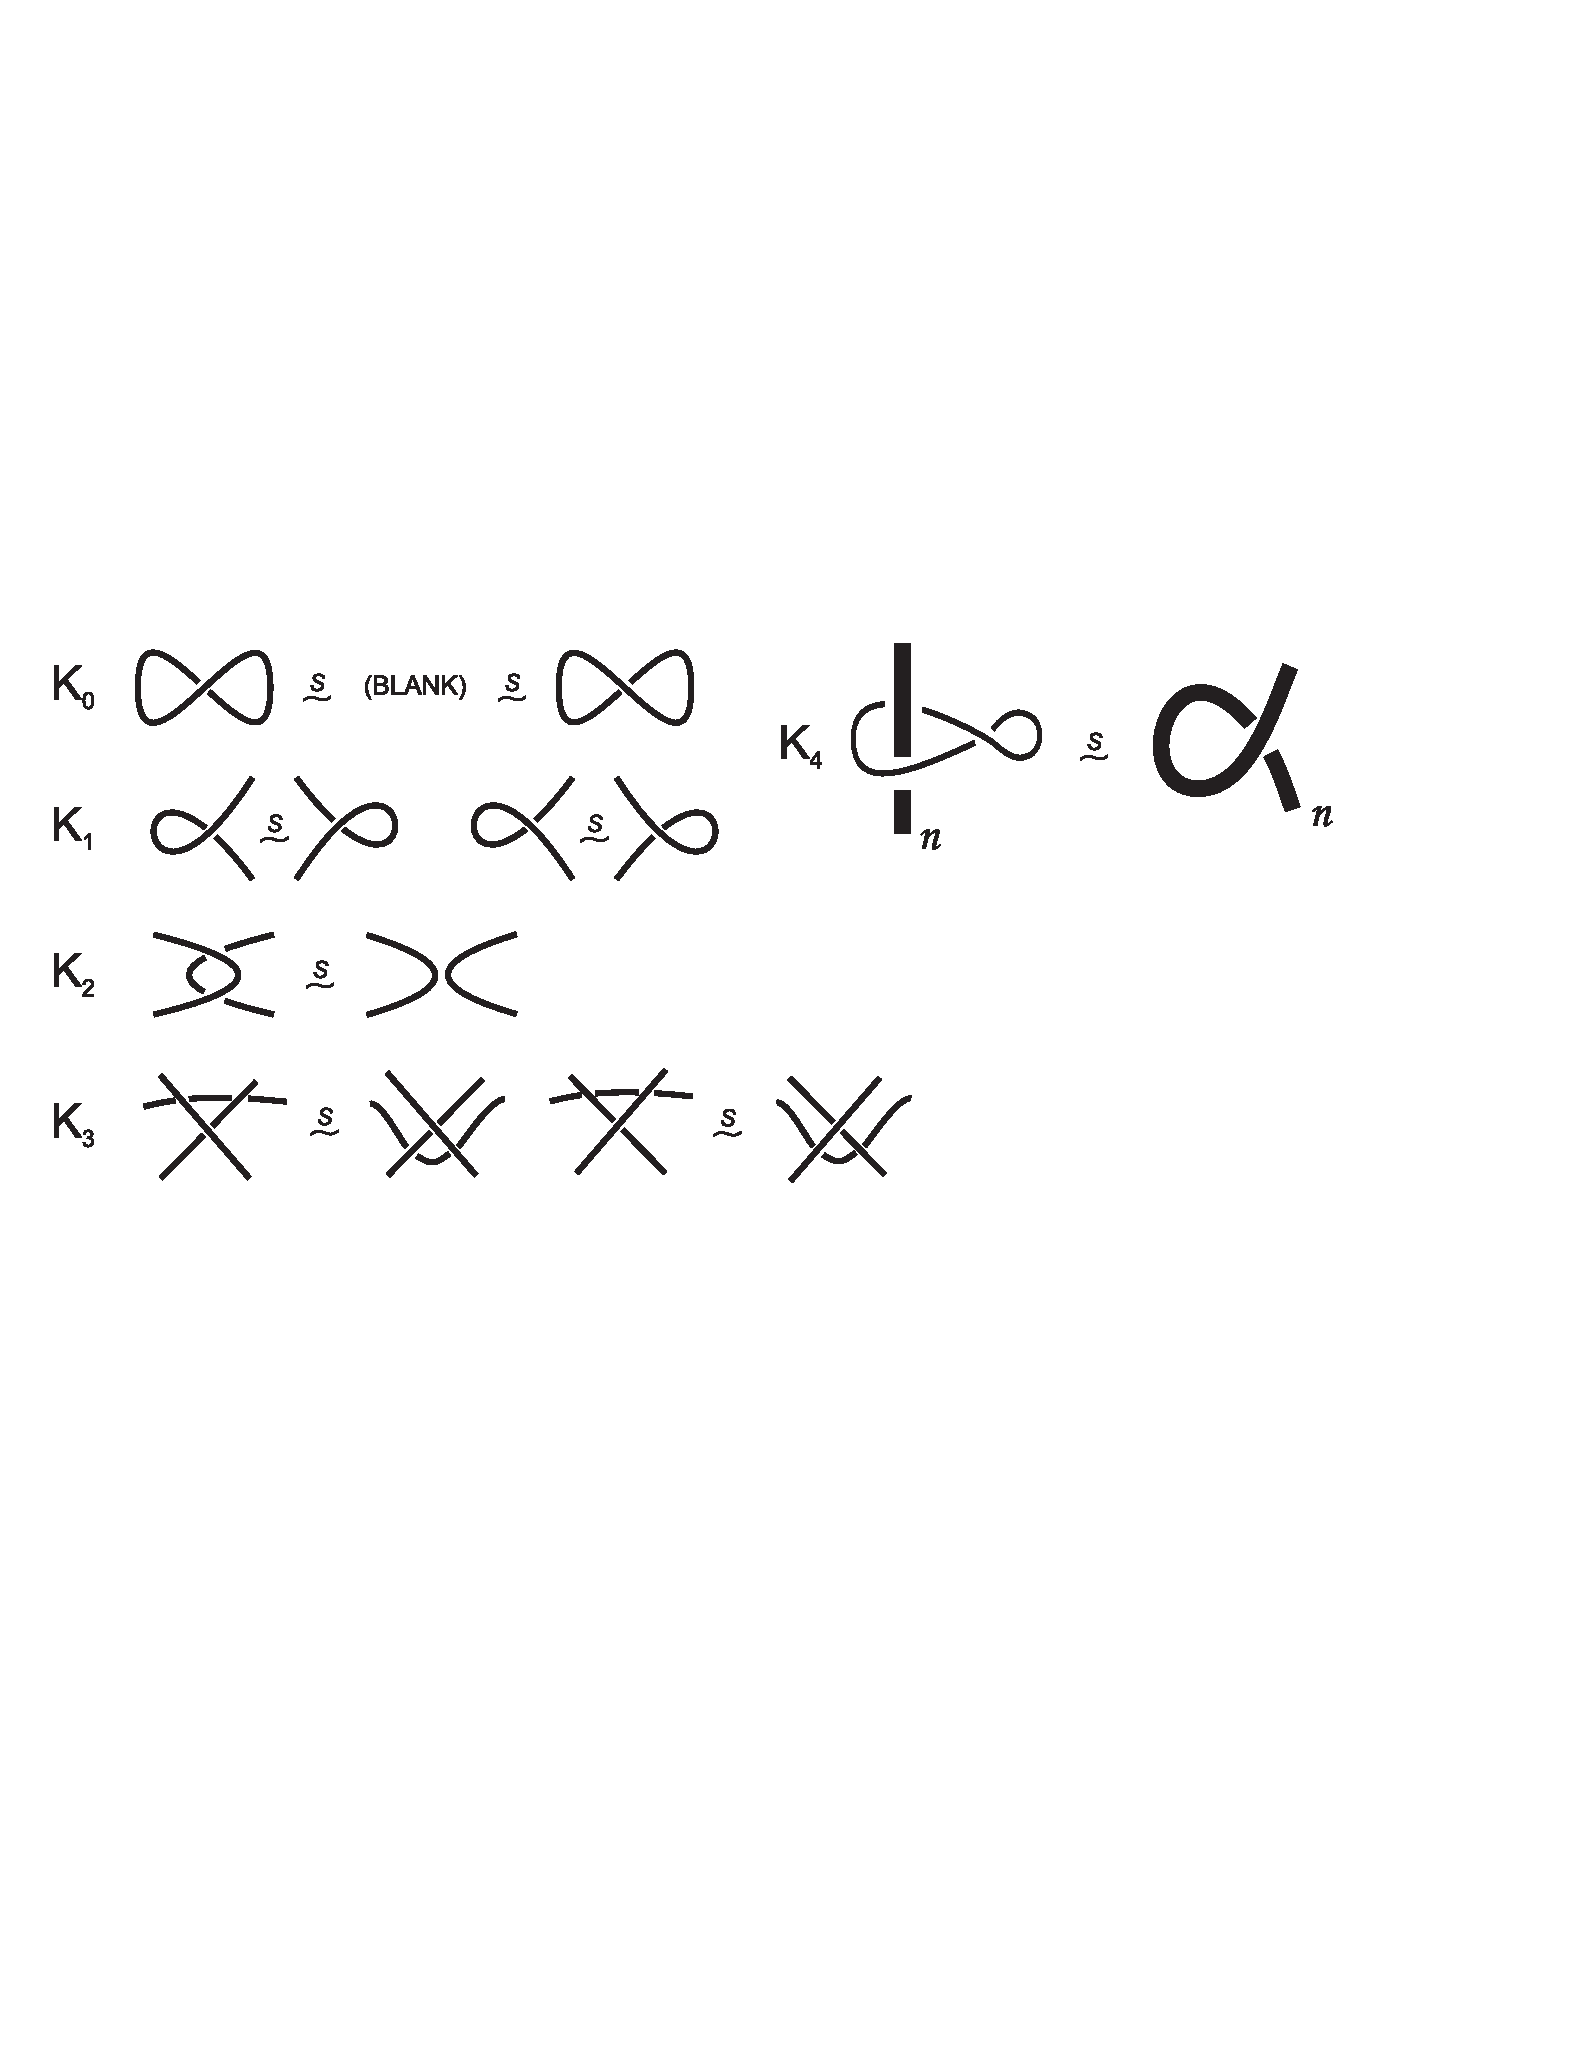
\includegraphics[width=12.5cm]{fig/BFLcalculusK1.eps}
   \end{center}
   \vspace{-0.7cm}
   \caption{ BFL calculus ${\cal K}^1$, obtained by replacing
   $K_5(n)$ by $K_1$ (ribbon move)}
   \label{fig:BFLcalculusK1}
\end{figure}

\pagebreak

We end this section with some results that are consequence of BFL calculus.

\begin{Lem}[Passing Wall Lemma] These patterns are all regular isotopic

\begin{center}
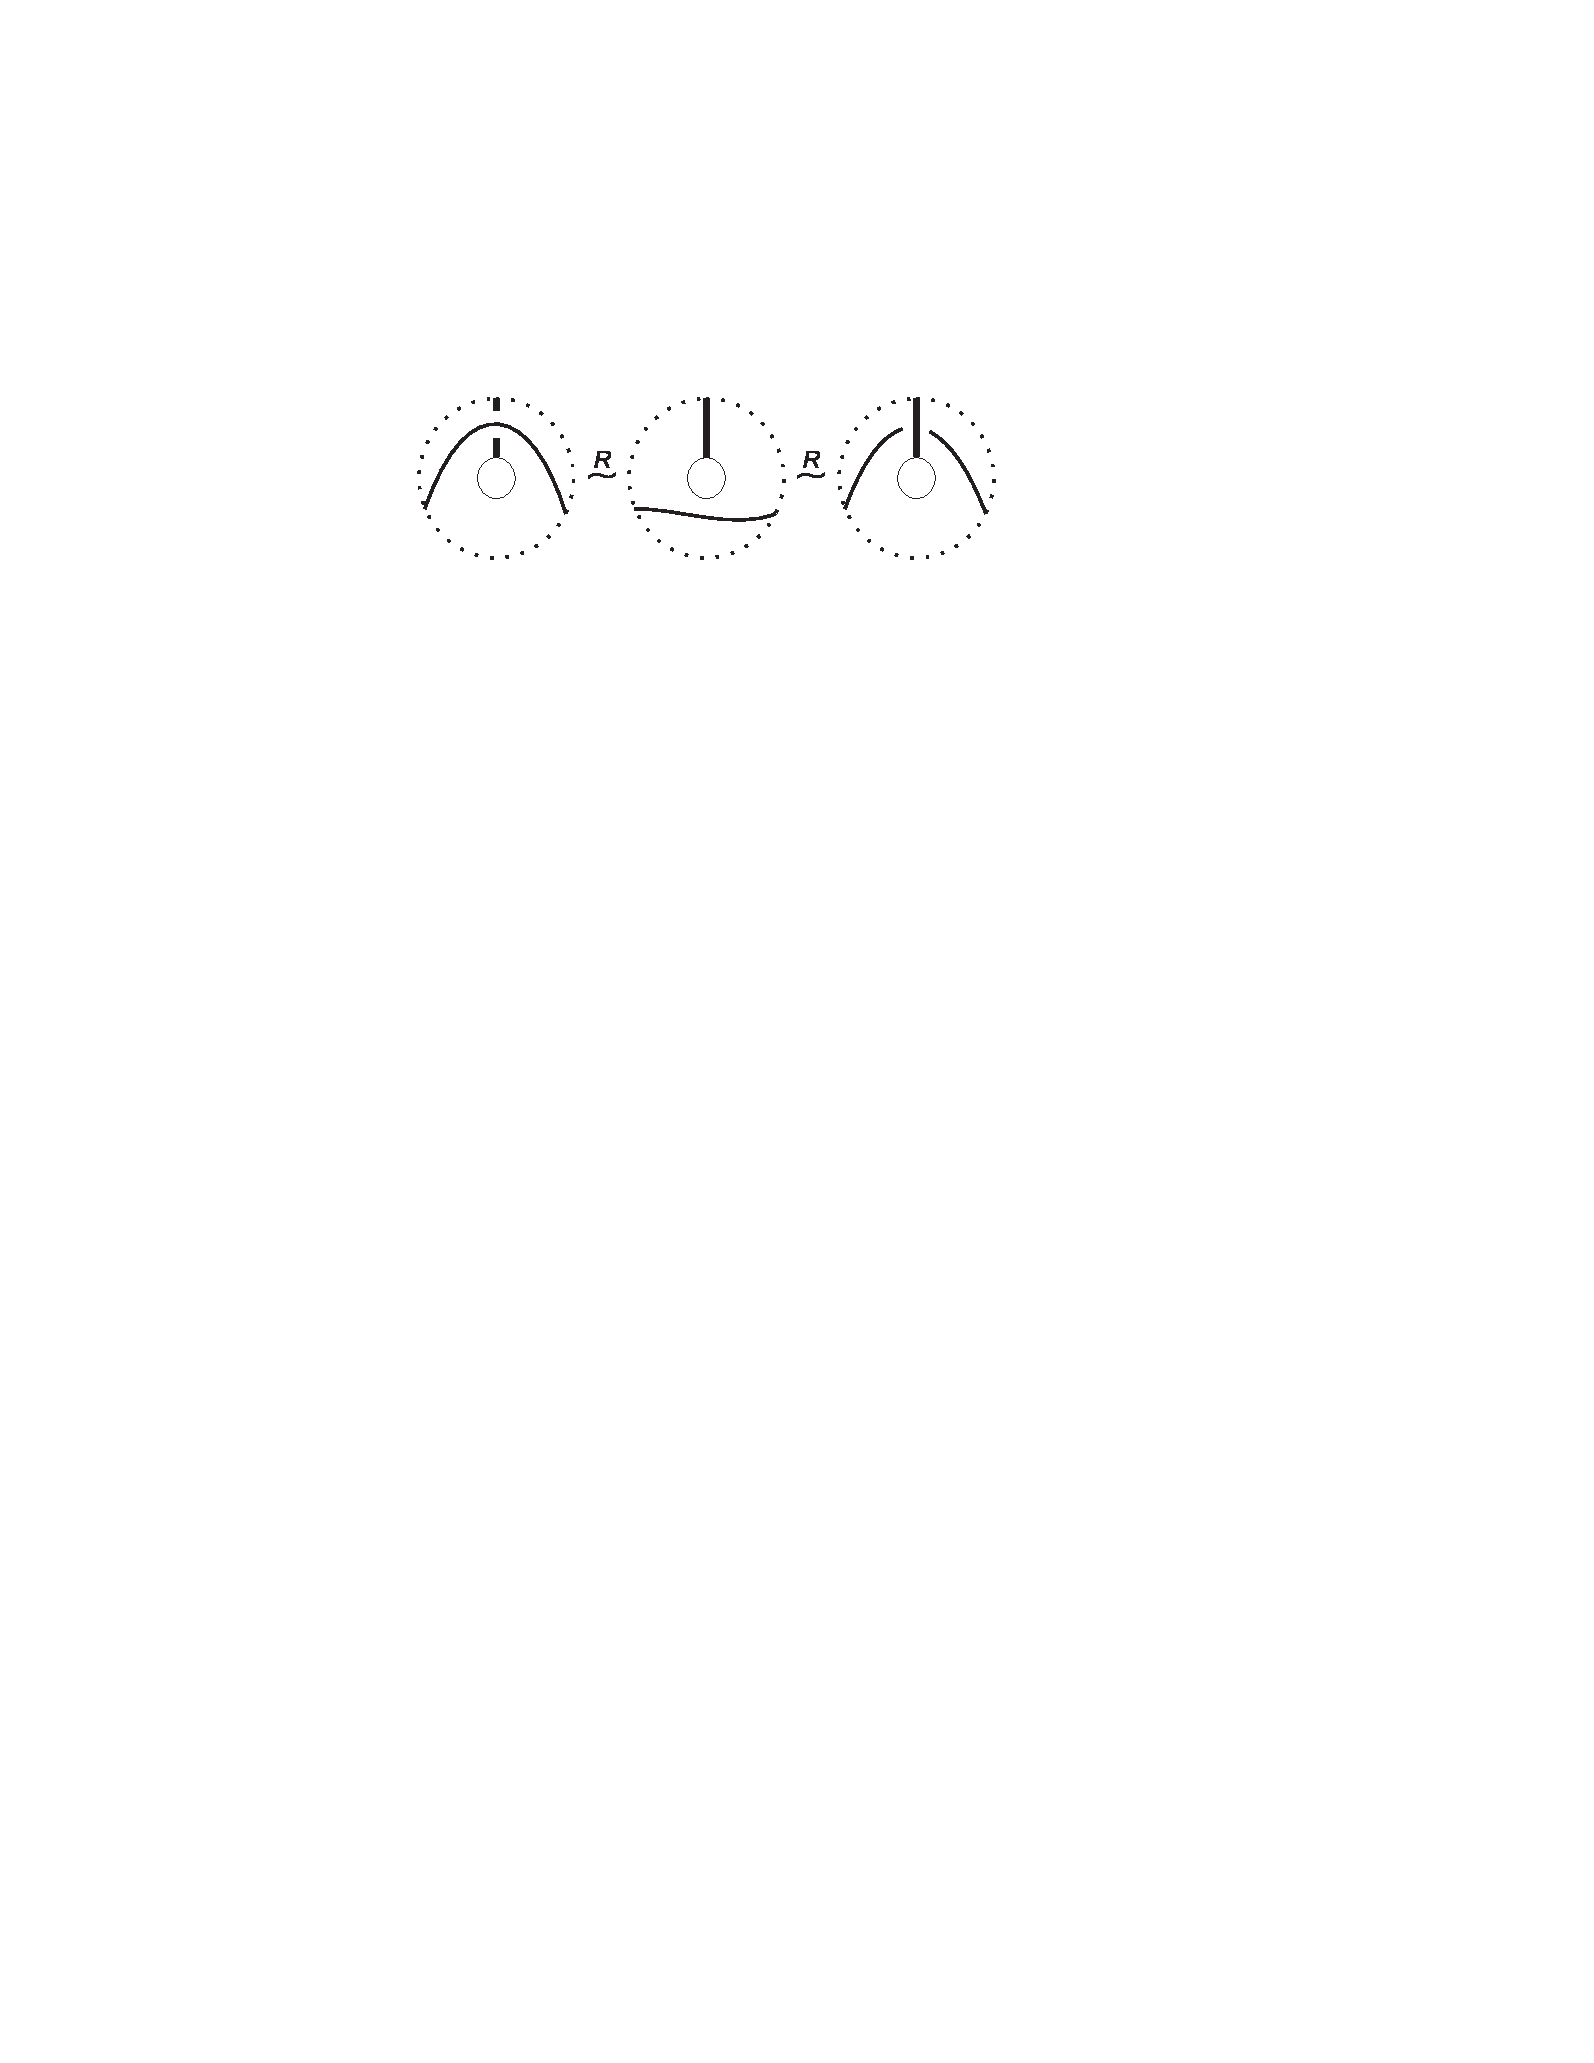
\includegraphics{fig/passingWallLemma.eps}
\end{center}
\end{Lem}
\begin{proof}
This is just the idea: start passing
the horizontal curve under xor (\ie exclusive or) over all
the crossings of the white ball using the moves $K_2$ and $K_3$.
\end{proof}

\begin{Lem}[Passing Cross Lemma] \label{lem:passingCrossLemma} The first
two and last two patterns are all regular isotopic
\begin{center}
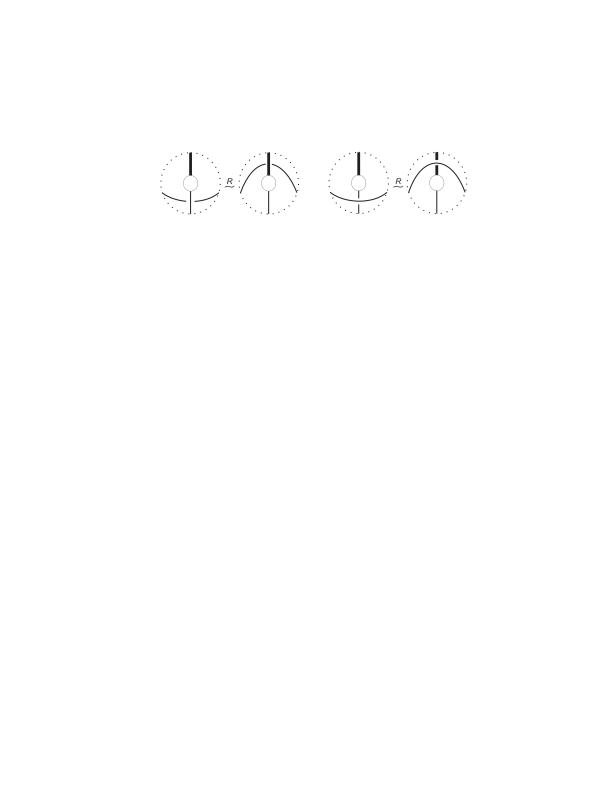
\includegraphics{fig/passingCrossLemma.eps}
\end{center}
\end{Lem}
\begin{proof} Follow the picture below. It proves that the first two
patterns of this lemma are regular isotopic. On the passage (1) the
pattern is rearranged to show the structure of the Passing Wall
Lemma. On passage (2) this lemma is applied. On passage (3) we use
the regular isotopy basic move $K_3$ and rearrange its result on
passage (4), arriving at the pattern wanted. The proof for the last
two pattern is analogous to this one.
\begin{center}
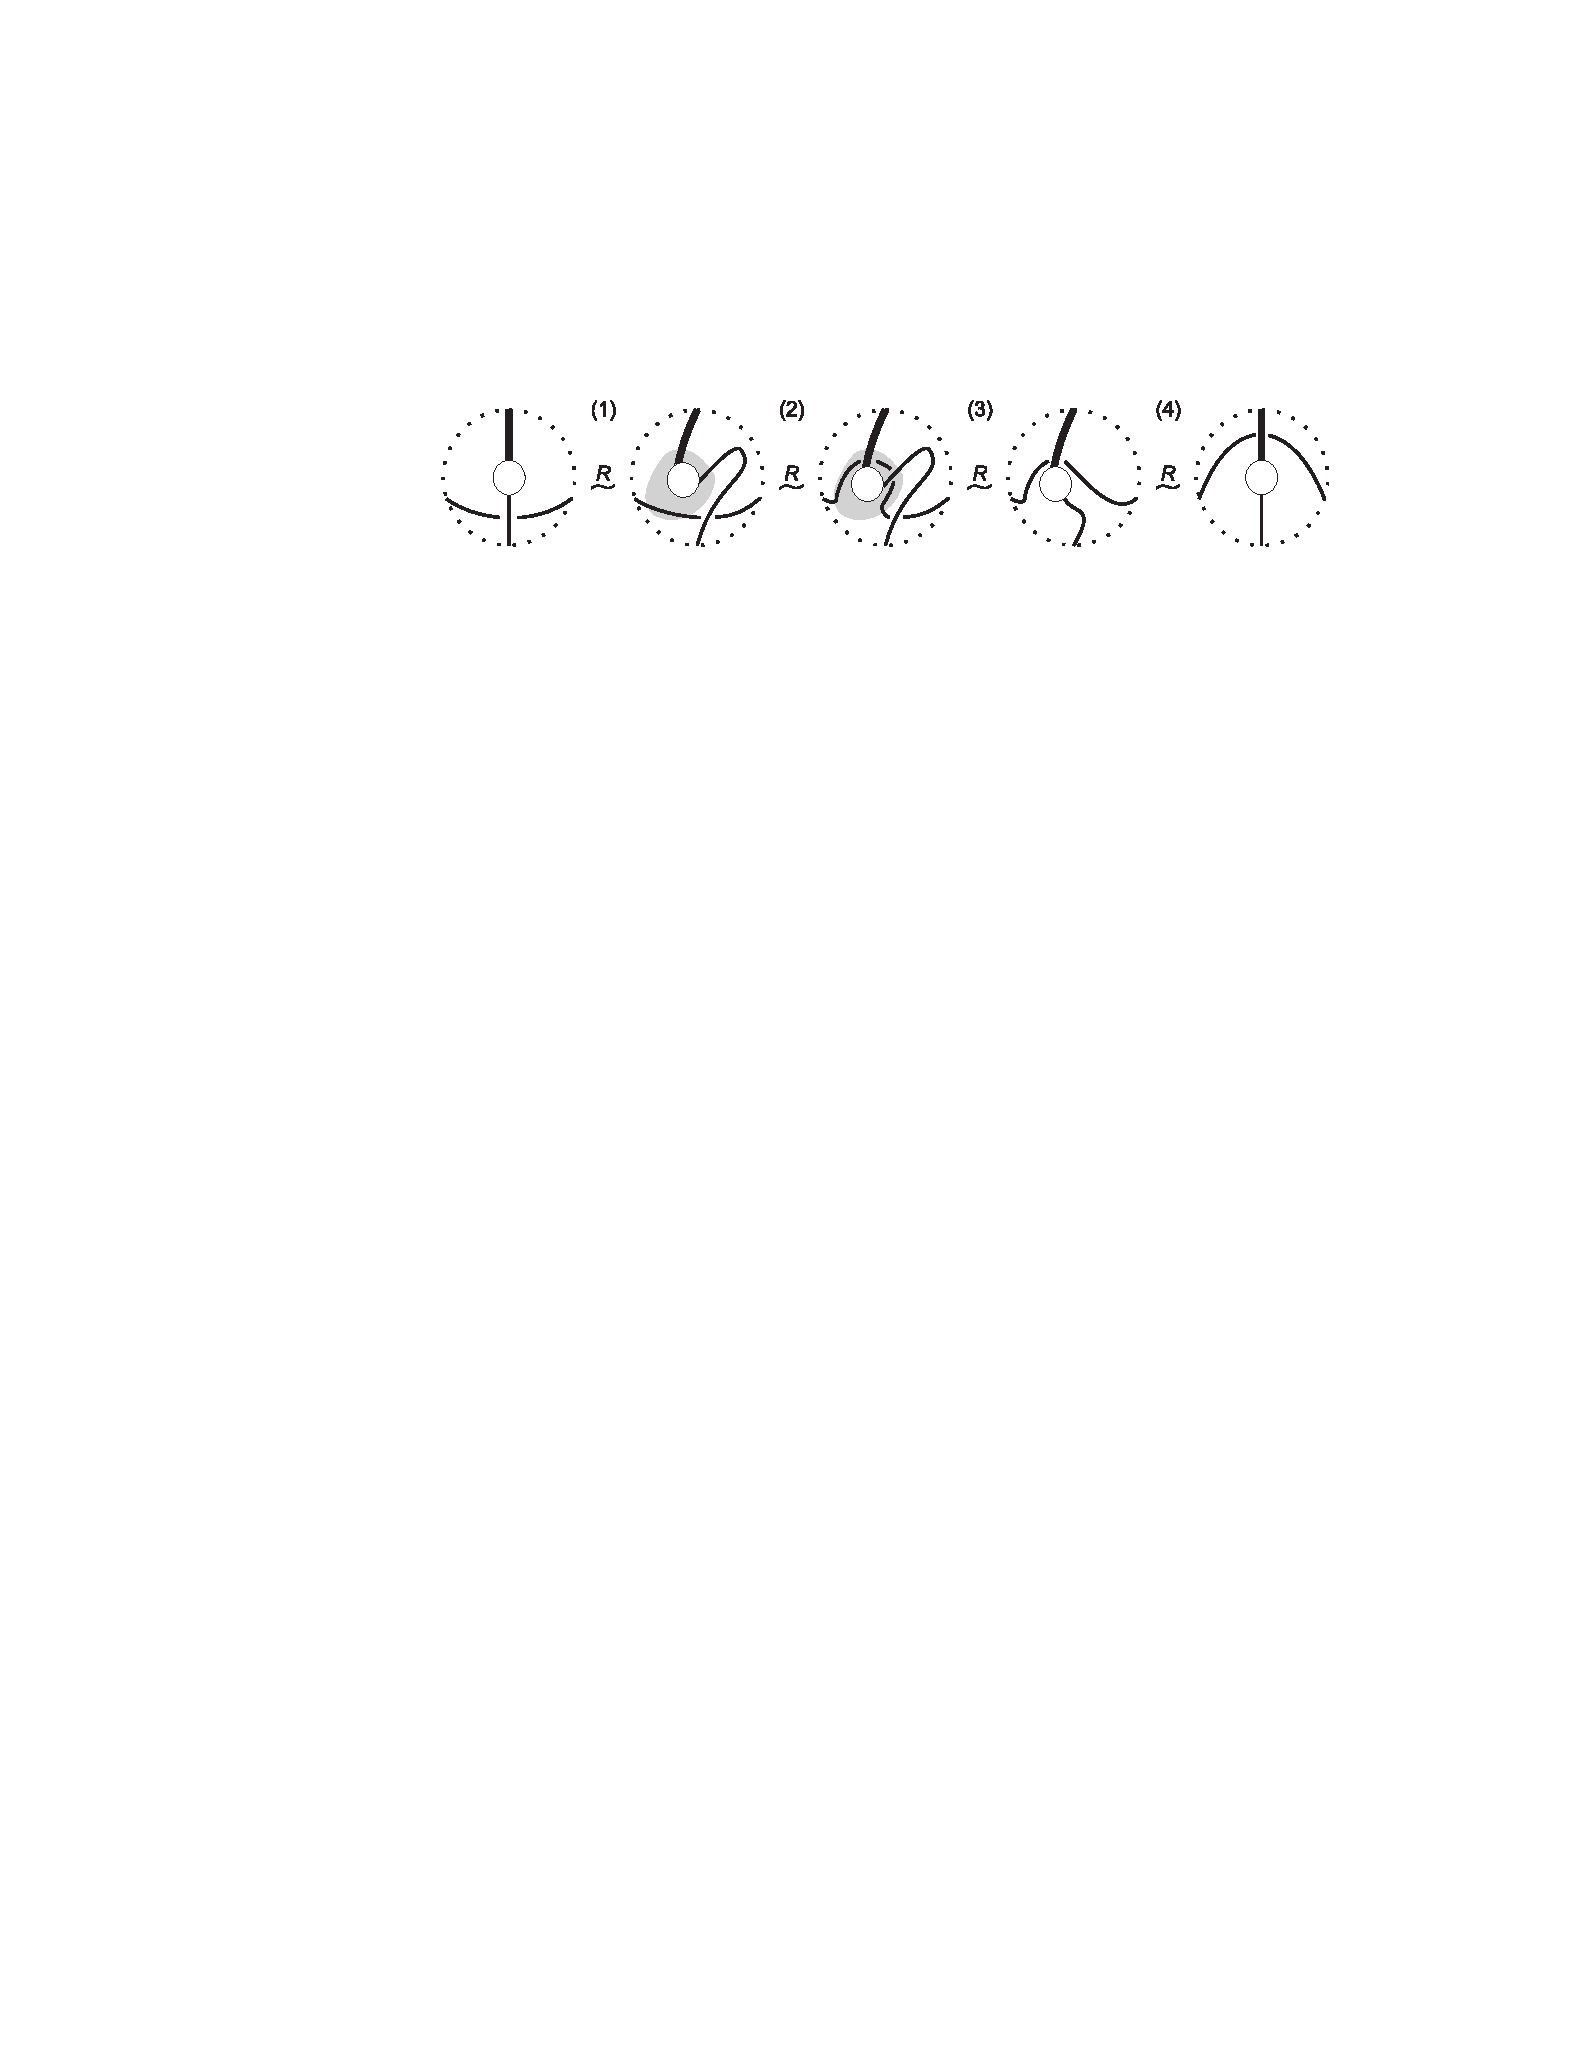
\includegraphics{fig/passingCrossLemmaProof.eps}
\end{center}
\end{proof}

\begin{Lem}[Jumping Rope Lemma] \label{lem:jumpingRopeLemma}
The following patterns induces the same space.
\begin{center}
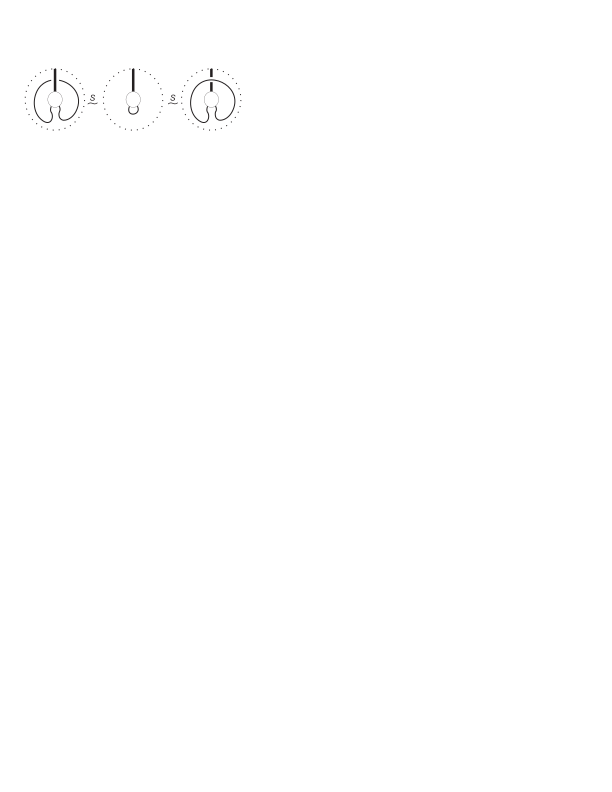
\includegraphics{fig/jumpingRopeLemma.eps}
\end{center}
\end{Lem}
\begin{proof} Follow the picture below. It proves that the first two
patterns of this lemma induce the same space. On the passage (1) the
pattern is rearranged to show the structure of the Passing Wall
Lemma. On passage (2) this lemma is applied. On passage (3) we just
rearrange the pattern to stress the two curls on the different sides
of the cable. On passage (4) the Passing Cross Lemma is repeatedly
applied until the right curl traverse all the cable. On passage (5)
the ribbon move is applied. Finally, the Whitney trick is used on
passage (6). We have thus proved that the first two patterns of this
lemma indeed induce the same space. From these steps it is clear how
the last pattern of this lemma is also proved to induce the same.
\begin{center}
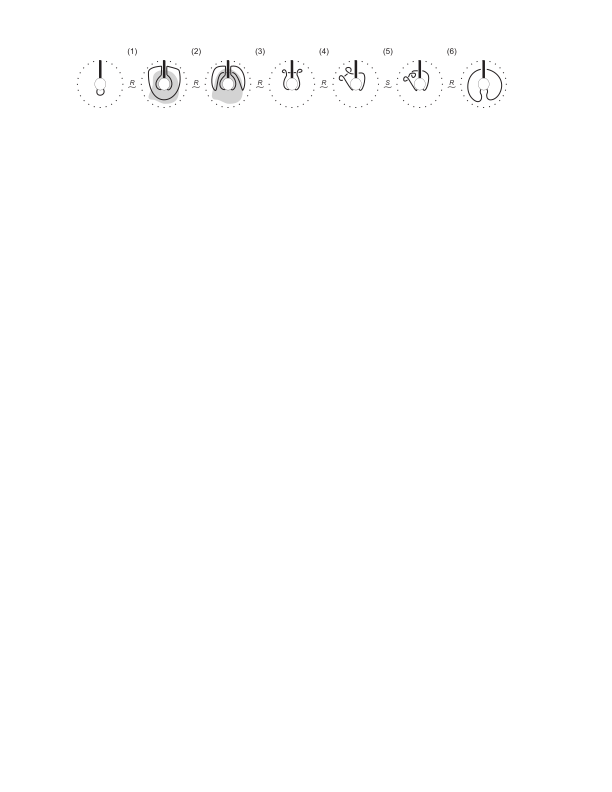
\includegraphics{fig/jumpingRopeLemmaProof.eps}
\end{center}
\vspace{-0.8cm}
\end{proof}


% \section{Invariants from Links}
